%% bantaylaot_paper.tex
%% BantayLaot+ IEEE Journal Paper
%% Updated with full Chapter 3 and Chapter 4 narratives

\documentclass[journal]{IEEEtran}

\usepackage{cite}

\ifCLASSINFOpdf
  \usepackage[pdftex]{graphicx}
  \graphicspath{{./figures/}{./figures/screenshots/}}
  \DeclareGraphicsExtensions{.pdf,.jpeg,.jpg,.png}
\else
  \usepackage[dvips]{graphicx}
  \graphicspath{{./figures/}{./figures/screenshots/}}
  \DeclareGraphicsExtensions{.eps}
\fi

\usepackage{amsmath}
\usepackage{booktabs}

\hyphenation{op-tical net-works semi-conduc-tor Ban-tay-La-ot}

\begin{document}

\title{BantayLaot+: An Enhanced System for Offline and Secure Monitoring of Philippine
Municipal Fisheries with AI Integration Preparedness}

\author{Magenta~Alarcon~and~Val~Randolf~Madrid}


\markboth{BantayLaot+: Enhanced Fisheries Monitoring System}%
{Alarcon \MakeLowercase{\textit{et al.}}: BantayLaot+ Enhanced System}

\maketitle

\begin{abstract}
Municipal fisheries monitoring in the Philippines is constrained by intermittent
internet connectivity, manual reporting workflows, and fragmented data infrastructure,
limiting the effectiveness of enforcement and research in coastal communities.
This paper presents BantayLaot+, an enhanced fisheries monitoring system targeting two
municipalities in Misamis Oriental, built on an offline-first mobile architecture that
stores session, catch, violation, and GPS data locally using Android's Room Database and
synchronizes records to a multi-tiered backend via WorkManager once network connectivity
is available. JWT authentication tokens are persisted in SharedPreferences to maintain
session continuity throughout extended field operations without connectivity dependency.
The system employs a structured image pipeline---compressing and uploading photographs
via Cloudinary---that lays the data foundation for future AI-assisted species
identification without requiring changes to the existing schema. Three
role-differentiated web dashboards, implemented in React.js and powered by a MERN
stack, serve municipal administrators, central administrators, and researchers with
jurisdiction-appropriate analytics including CPUE summaries, GPS route visualization
via OpenLayers, and anonymized registration and catch statistics. Usability was
evaluated using the System Usability Scale (SUS) with fifteen respondents distributed
across three user groups. Results indicate that BantayLaot+ addresses the offline
reliability, authentication continuity, and structured data collection gaps identified
in the predecessor system, and establishes the infrastructure required for future
AI model integration.
\end{abstract}

\begin{IEEEkeywords}
fisheries monitoring, offline-first architecture, Android, WorkManager, Room Database,
MERN stack, CPUE, IUU fishing, municipal fisheries, Philippines
\end{IEEEkeywords}

\IEEEpeerreviewmaketitle

%% ============================================================
%% SECTION I — INTRODUCTION
%% ============================================================

\section{Introduction}

The Philippines, an archipelagic nation with over 36,000 kilometers of coastline, depends profoundly on its marine resources for economic sustenance, food security, and cultural identity. Fisheries, particularly small-scale and municipal operations, serve as a primary livelihood for millions of coastal households, contributing significantly to national nutrition and local economies (Food and Agriculture Organization [FAO], 2023). However, the sustainability of these resources is increasingly jeopardized by illegal, unreported, and unregulated (IUU) fishing activities. According to the World Wildlife Fund (2022), IUU fishing undermines fish stock recovery, distorts market dynamics, and erodes the ecological integrity of marine habitats, especially in municipal waters where enforcement capacity is often limited.

Efforts to curb IUU fishing have traditionally relied on manual reporting, sporadic patrols, and centralized data systems, which are often inaccessible to remote communities. These limitations have prompted a shift toward digital interventions that promote participatory monitoring and decentralized data collection. Technological innovations, particularly mobile and web-based platforms, offer scalable solutions for enhancing transparency, accountability, and responsiveness in fisheries governance.

In response to these challenges, BantayLaot was developed as a community-oriented digital system designed to assist both government agencies and fisherfolk in reporting fish catch data, tracking vessel movements, and documenting IUU violations \cite{Gallero2025}. The system leveraged mobile and web technologies to provide GPS-based session tracking, fish catch documentation, and offline data storage, alongside a web platform for CPUE analysis and geospatial visualization. Initial evaluation confirmed its foundational functionality; however, testing revealed several operational gaps: the absence of an account and authentication system, a single-role web interface with no differentiation between administrator tiers or researchers, lack of structured synchronization state management, and no organized image pipeline for future analytical use. These shortcomings are particularly relevant in geographically isolated coastal areas, where extended offline operation and multi-stakeholder data access are operational requirements.

To address these gaps, this study proposes BantayLaot+, an enhanced version of the original system. BantayLaot+ introduces JWT-based authentication with locally persisted tokens for offline session continuity, a structured WorkManager synchronization pipeline with per-record state tracking, a multi-tiered server architecture separating per-municipality and central data stores, role-differentiated web dashboards for municipal administrators, central administrators, and researchers, and a structured image collection pipeline designed to support future AI-assisted species identification. By aligning architectural design with the operational realities of coastal communities, BantayLaot+ aspires to strengthen fisheries monitoring and support sustainable resource management.

\subsection{Statement of the Problem}

The existing BantayLaot system lacks an account and authentication system, role-based access control, structured synchronization state management, and a multi-tiered data architecture, limiting its suitability for multi-stakeholder operational use. There is a need for an enhanced, securely designed system with a structured image pipeline that lays the groundwork for future AI integration, to enable more reliable and scalable fisheries monitoring.

\subsection{Objectives of the Study}

This study aims to enhance the existing BantayLaot system by improving its mobile application, web application, and database/backend infrastructure to support more efficient, secure, and scalable field operations. Specifically, the study seeks to:

\begin{enumerate}
\item Enhance the mobile application with improved usability, JWT-based authentication, structured offline data storage with per-record synchronization state tracking, and a structured image collection pipeline designed to support future AI-assisted fish species identification, while retaining manual species and weight input.
\item Develop a secure multi-tiered database with per-municipality local storage and a central cloud instance, along with role-differentiated web dashboards for municipal administrators, central administrators, and researchers, with a data schema designed to accommodate future AI integration without structural changes.
\item Test and deploy the enhanced system in real-world monitoring environments to evaluate performance, usability, system reliability, and suitability for operational use.
\end{enumerate}

\subsection{Significance of the Study}

BantayLaot+ serves three primary stakeholder groups. Fisherfolk gain a more reliable
field tool with offline catch and violation reporting, continuous GPS tracking, and an
interface designed for varying digital literacy levels. Municipal and central government
agencies benefit from structured, role-based access to catch logs, violation records, and
CPUE analytics, supporting evidence-based enforcement. Researchers access anonymized
aggregated datasets through a dedicated dashboard, enabling fisheries trend analysis and
conservation research without exposing fisher identities. Collectively, these contributions
support Sustainable Development Goal (SDG) 14: \textit{Life Below Water} through improved
marine resource monitoring and conservation, and SDG 11: \textit{Sustainable Cities and
Communities} by strengthening data-driven coastal governance and sustainable local
livelihood management.

\subsection{Scope and Limitations}

This study covers the development and evaluation of BantayLaot+, targeting two
municipalities in Misamis Oriental for future deployment. The mobile application (Android/Kotlin) supports offline catch
and violation reporting, continuous GPS tracking, and background data synchronization to
locally hosted municipal servers. The web platform (React.js) provides dashboards for municipal administrators, central
administrators, and researchers, with analytics including CPUE analysis, violation
summaries, and GPS session visualization using OpenLayers.

A multi-tiered database architecture is used: per-municipality MongoDB instances running
on local servers (localhost) at each municipality, and a central cloud MongoDB database
deployed on Railway. Images are stored via Cloudinary. All species, gear, and weight
inputs are entered manually; image data collected during deployment provides the
foundation for future AI model training.

Limitations include image quality variability affecting future AI model training, device
hardware differences affecting GPS precision, small respondent pool (15 total across
three user groups), and time constraints limiting evaluation under extreme connectivity
conditions.

%% ============================================================
%% SECTION II — REVIEW OF RELATED LITERATURE
%% ============================================================

\section{Review of Related Literature}

\subsection{BantayLaot: The Predecessor System}

BantayLaot, developed by Gallero \cite{Gallero2025}, established the foundational
concept of a mobile-assisted fisheries monitoring platform for Philippine municipal
waters. The system enabled fisherfolk to document catch records, submit IUU violation
reports, and log GPS-tracked fishing sessions via a Kotlin mobile application, with
offline storage through Room Database and synchronization to a MERN stack backend.
Its single web dashboard provided CPUE analysis, geospatial route visualization using
OpenLayers, and violation summaries for administrative review. The system was evaluated
through laboratory testing using simulated data, and this evaluation surfaced the
operational constraints---absence of an account and authentication system, a single
undifferentiated administrative role, lack of structured sync state management, and no
organized image pipeline---that BantayLaot+ directly addresses. This work builds upon
and extends that foundation.

\subsection{Offline-First Architecture and Session Persistence}

Field-based systems in low-connectivity environments require offline-first designs that
store data locally and synchronize when network access is restored \cite{Serrano2020}.
BantayLaot+ implements this using Android's Room Database for local SQLite storage of
fishing sessions, catches, violation reports, and GPS tracks. Session continuity is maintained through JWT tokens stored in SharedPreferences,
enabling continued app access without repeated server authentication. Dahiru and Ibrahim (2021) validate this
approach for secure mobile systems operating under intermittent connectivity
\cite{Dahiru2021}.

\subsection{Background Synchronization}

WorkManager is the recommended Android framework for deferred, constraint-aware background
tasks \cite{Google2022}. BantayLaot+ uses it to automatically upload catch logs, GPS
tracks, violation reports, and images to municipal servers once network connectivity is
available. Timestamp-based conflict resolution, as recommended by Kumar and
Singh (2020), ensures consistency across records submitted from different devices
\cite{Kumar2020}. Goncalves et al. (2020) confirm that background synchronization
significantly reduces data loss in field-deployed mobile applications with variable
connectivity \cite{Goncalves2020}.

\subsection{MERN Stack and Multi-Role Web Dashboards}

The MERN stack (MongoDB, Express.js, React.js, Node.js) supports scalable, real-time
data platforms \cite{Chodorow2013}. BantayLaot+ uses this stack to deliver three
role-differentiated dashboards: municipal administrators manage jurisdiction-level catch
and violation data; central administrators access aggregated cross-municipality analytics;
researchers view anonymized datasets for analysis. API-driven architectures support
secure, multi-role data access across independent municipality servers \cite{Alzubaidi2020}.

\subsection{Geospatial Visualization}

OpenLayers, paired with OpenStreetMap tiles, provides a lightweight and extensible web
mapping solution suitable for tracking and spatial analysis \cite{Haklay2008}.
BantayLaot+ uses OpenLayers to render GPS session routes and violation incident locations
on the web dashboard, enabling both operational review and geographic pattern detection.

\subsection{Image-Based Documentation and AI Preparedness}

Structured image capture and organized storage are foundational for future machine
learning applications in species identification \cite{Norouzzadeh2018}. BantayLaot+
captures images for fish catches, vessel documentation, and violation evidence, storing
them via Cloudinary with metadata linking to sessions and users. This repository supports
future AI model training while all current inputs remain manual.

%% ============================================================
%% SECTION III — METHODOLOGY
%% ============================================================

\section{Methodology}

This study followed an iterative, feature-driven development approach
aligned with agile principles. Development was organized into sequential sprints, each
targeting a discrete system component: the offline-first mobile architecture, background
synchronization, JWT-based authentication, the mobile View Binding interface,
per-municipality and central REST APIs, and the role-differentiated web dashboards. Each
sprint concluded with integration testing before the next phase was initiated, allowing
defects and architectural inconsistencies to be identified and resolved incrementally.
The evaluation phase applied the System Usability Scale (SUS) to representative
respondents from three user groups following system development and testing targeting
two municipalities in Misamis Oriental.

\subsection{Technology Specifications}

Development was conducted on machines running Windows 11 with Intel Core i5 processors
and 16~GB RAM. This configuration was sufficient for running the Android emulator, local
Node.js server instances, and MongoDB simultaneously during development and integration
testing.

\subsection{Development Tools}

The technology stack was selected to meet the system's requirements for offline operation,
multi-role access, and geospatial visualization. Visual Studio Code served as the primary
editor for backend and web development. Android Studio was used for mobile development,
compilation, and device emulation. The mobile application was written in Kotlin using
traditional Android Views with View Binding for layout construction, enabling direct
access to UI elements while maintaining clear separation of layout and logic.

The backend and web interface were built on the MERN stack. MongoDB provides
document-oriented storage suited to the variable structure of catch records, violation
reports, and GPS tracks. Express.js serves as the REST API framework across both the
municipal and central server instances. React.js powers the web dashboards, and Node.js
handles server-side processing and synchronization logic. OpenLayers paired with
OpenStreetMap tiles provides the map rendering layer for GPS session routes and violation
incident locations. On mobile, Android Location Services handles continuous GPS
acquisition, and WorkManager governs deferred background synchronization subject to
network connectivity constraints. Room Database manages local SQLite storage on the device, and SharedPreferences
provides secure JWT token persistence for offline authentication continuity. Cloudinary, integrated via Multer
middleware, handles image upload and cloud storage.

\subsection{System Architecture}

BantayLaot+ employs a multi-tiered architecture comprising five functional layers:
client, API, processing, data, and external services, as illustrated in
Fig.~\ref{fig:system_architecture}.

\begin{figure}[h]
    \centering
    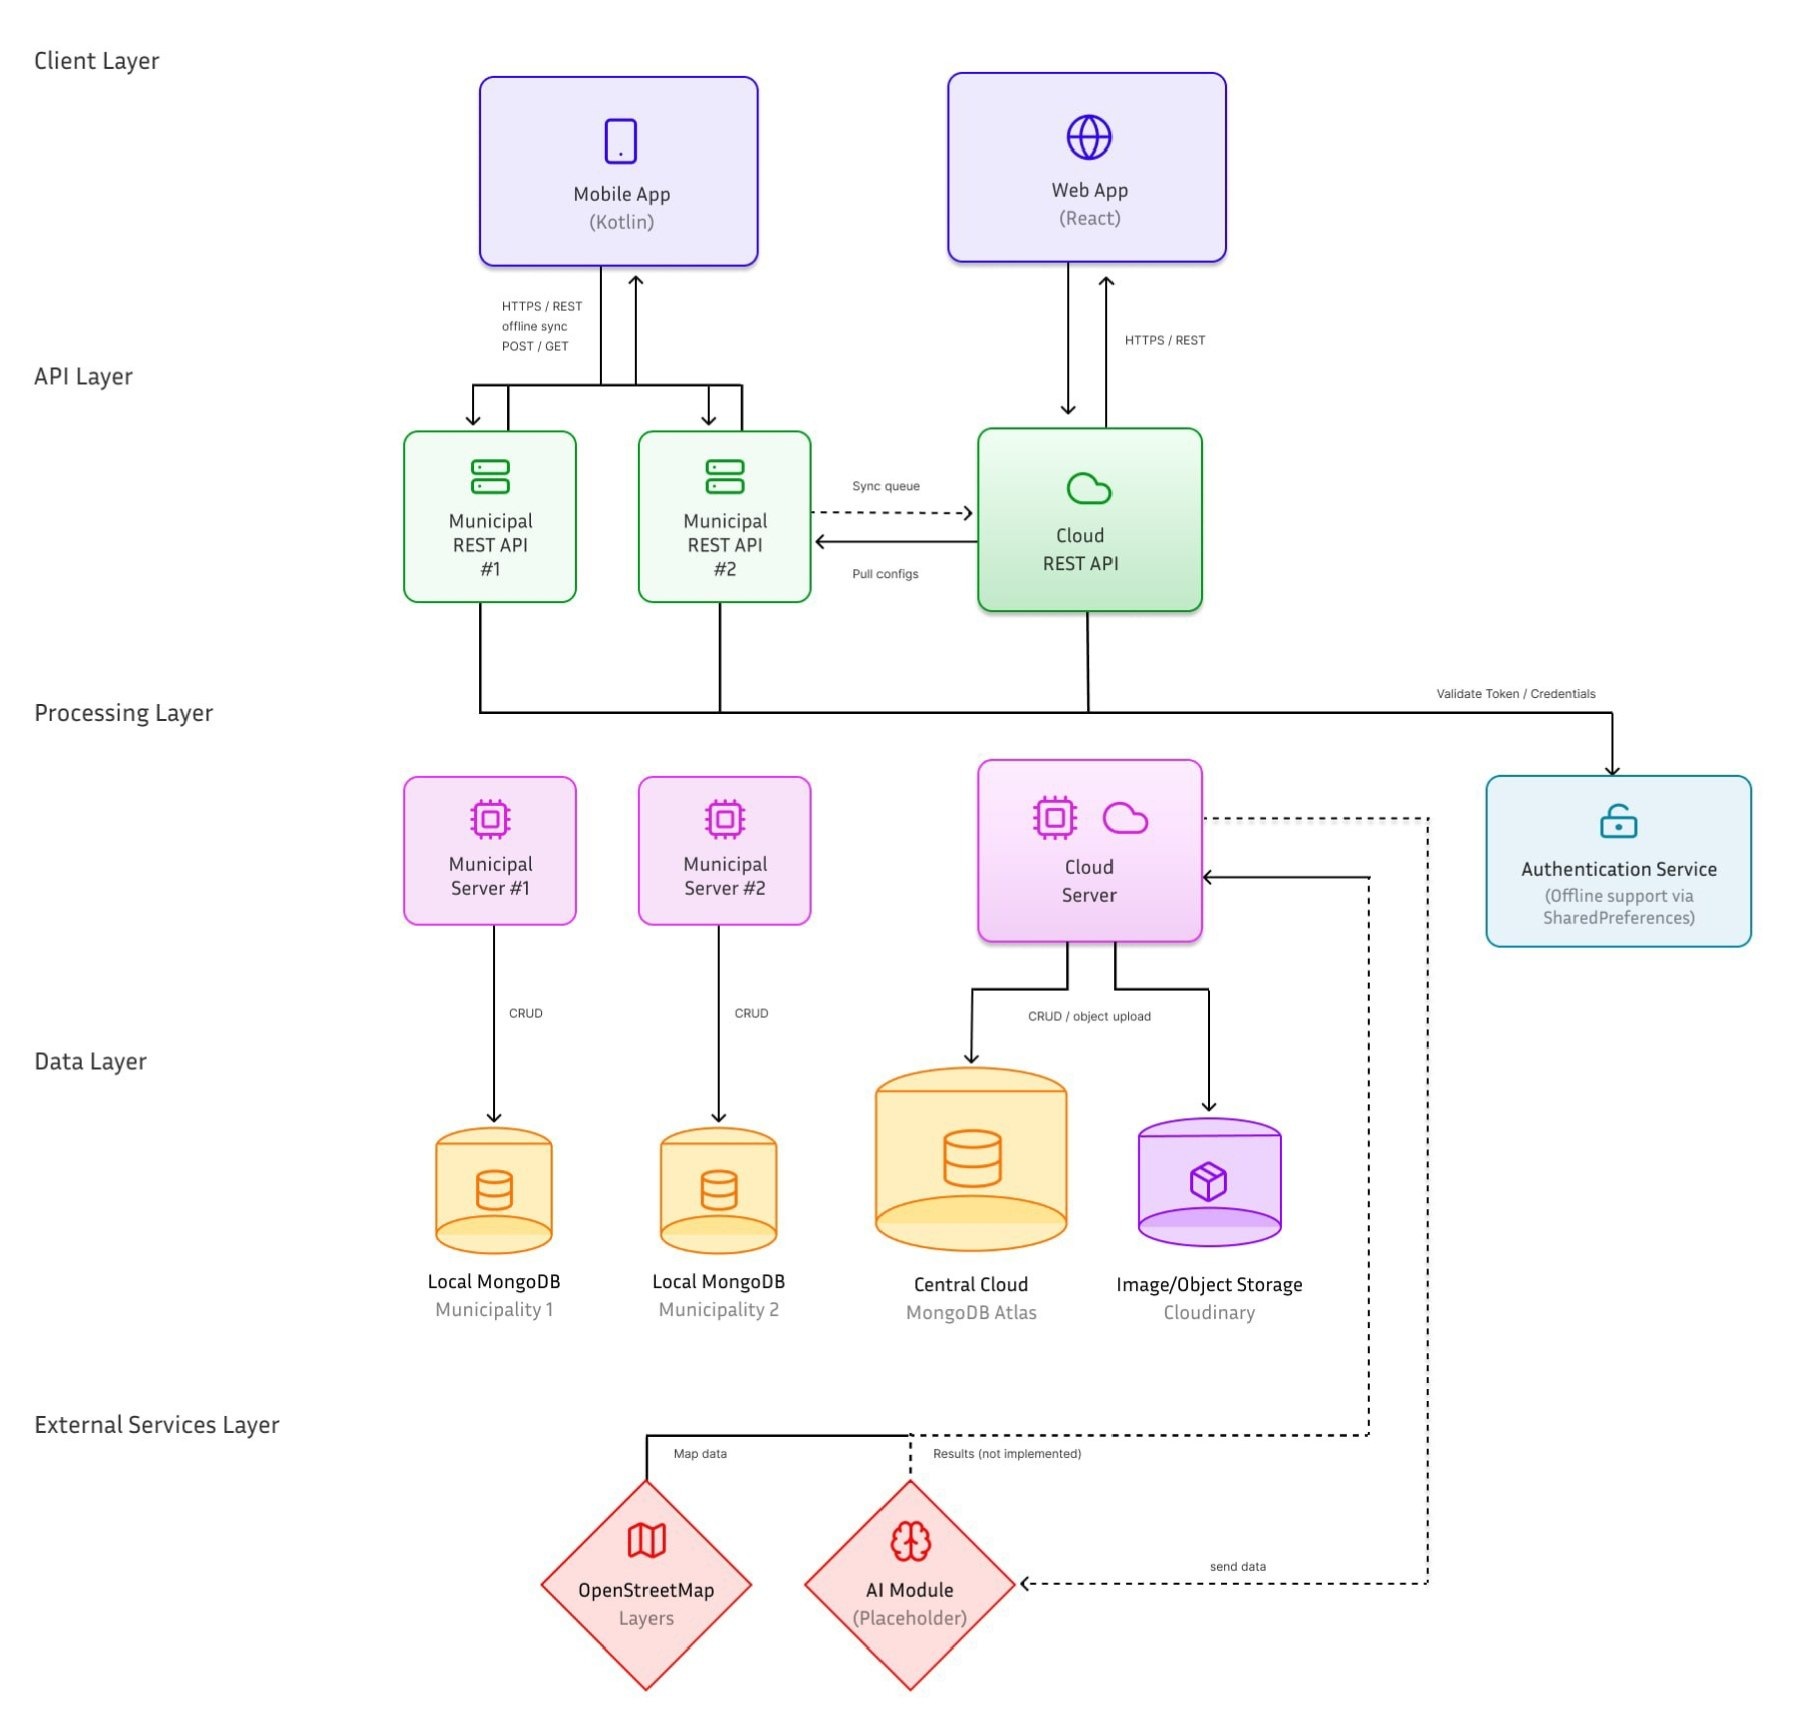
\includegraphics[width=0.45\textwidth]{system_architecture.jpg}
    \caption{BantayLaot+ Multi-Tiered System Architecture}
    \label{fig:system_architecture}
\end{figure}

The \textit{client layer} consists of the Android mobile application (Kotlin) and the
React.js web application. The mobile app communicates with the municipal REST APIs via
HTTPS/REST for offline-aware data submission (POST/GET), with all records written locally
first and transmitted once connectivity is available. The web application communicates
with the cloud REST API via HTTPS/REST for cross-municipality analytics and user
management.

The \textit{API layer} comprises two municipal REST API servers deployed on local
machines at each municipality and a central cloud REST API. The municipal APIs handle
authentication, CRUD operations for catch logs, violation reports, and GPS tracks, and
receive batched uploads from mobile clients during synchronization. Synchronized records
are forwarded to the cloud REST API via a sync queue, and configuration parameters are
pulled back from the cloud server to keep municipal instances consistent.

The \textit{processing layer} contains three server components and a dedicated
authentication service. Municipal Server~\#1 and Municipal Server~\#2 handle
jurisdiction-scoped data processing for their respective municipalities, while the Cloud
Server manages cross-municipality data aggregation. The Authentication Service validates
tokens and credentials for all incoming requests and provides offline authentication
support through SharedPreferences on the mobile client, allowing the app to
remain accessible without a live server connection during extended field operations.
WorkManager governs synchronization scheduling on the mobile side, queuing uploads
subject to network availability and retrying failed transfers automatically.
Timestamp-based conflict resolution at the cloud server ensures consistency when records
from different devices overlap.

The \textit{data layer} consists of per-municipality local MongoDB instances for
jurisdiction-scoped operational data and a central MongoDB Atlas instance in the cloud
for aggregated analytics and researcher access. Fish, vessel, and violation images are
stored in Cloudinary (Image/Object Storage), with metadata linking each asset to its
associated session, user, and record.

The \textit{external services layer} encompasses OpenStreetMap, which supplies map tile
data for GPS route visualization in the web dashboards via OpenLayers, and an AI Module
placeholder that represents the intended future integration point for AI-assisted species
identification. The AI Module is not implemented in the current version; the data
pipeline and schema are structured to accommodate it without requiring architectural
changes when the module is developed.

\subsection{Use Case Scenarios}

\subsubsection{Mobile Application Use Case}

The mobile workflow is structured around four operational stages corresponding to a
typical fishing trip, as depicted in Figs.~\ref{fig:pre_departure}--\ref{fig:synchronization}.

\paragraph{Pre-Departure}
As shown in Fig.~\ref{fig:pre_departure}, the fisherfolk authenticates using locally
persisted JWT credentials, eliminating dependency on server availability at login time.
Upon successful authentication, the user initiates a new fishing session. GPS tracking is
initialized via Android Location Services, and Room Database prepares local storage
partitions for the session, catch, violation, and GPS track records associated with that
trip.

\begin{figure}[h]
    \centering
    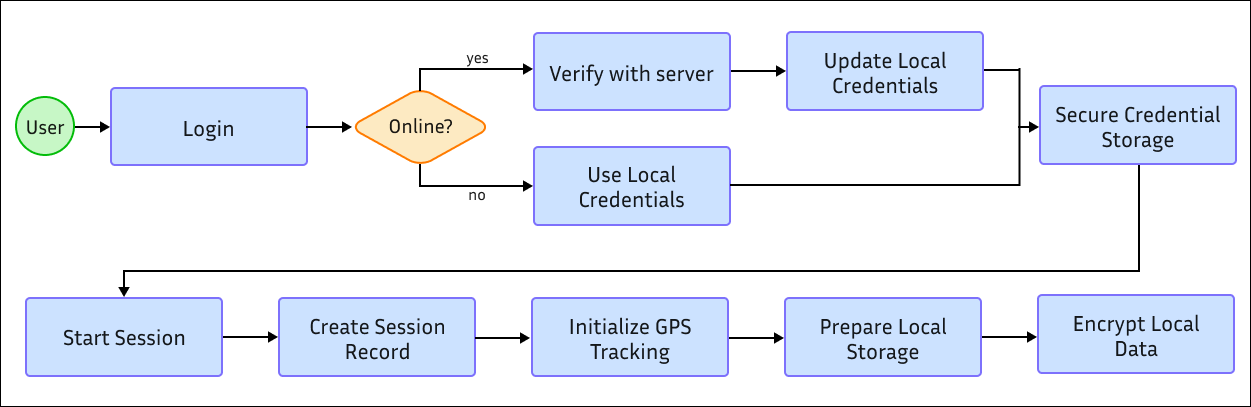
\includegraphics[width=0.45\textwidth]{Pre-Departure.png}
    \caption{Pre-departure stage use case flow}
    \label{fig:pre_departure}
\end{figure}

\paragraph{At Sea}
Fig.~\ref{fig:at_sea} illustrates the at-sea stage, during which GPS coordinates are
recorded every 30 seconds and written to Room Database regardless of connectivity state.
Fisherfolk may submit violation reports at any point by capturing a geotagged photo and
manually entering the violating vessel description, gear type, and incident narrative.
Violation coordinates are automatically attached from the current GPS fix, and all records
are stored locally with PENDING synchronization status.

\begin{figure}[h]
    \centering
    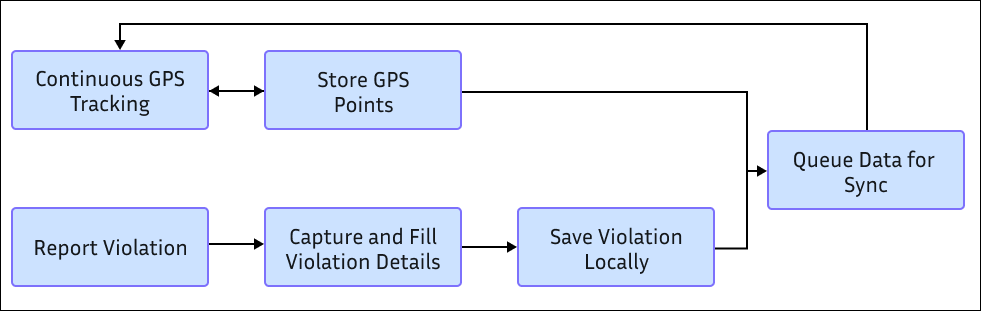
\includegraphics[width=0.45\textwidth]{At Sea.png}
    \caption{At-sea stage use case flow}
    \label{fig:at_sea}
\end{figure}

\paragraph{Returning to Shore}
As depicted in Fig.~\ref{fig:landing}, upon returning to shore, fisherfolk document
catches by photographing each haul and manually selecting the species from an
autocomplete dropdown of 975 recognized Philippine species, entering weight in kilograms,
and selecting one of three gear categories: Surface Gill Net, Bottom Set Gill Net, or
Hook and Line. Completed catch records are appended to the session and marked PENDING.

\begin{figure}[h]
    \centering
    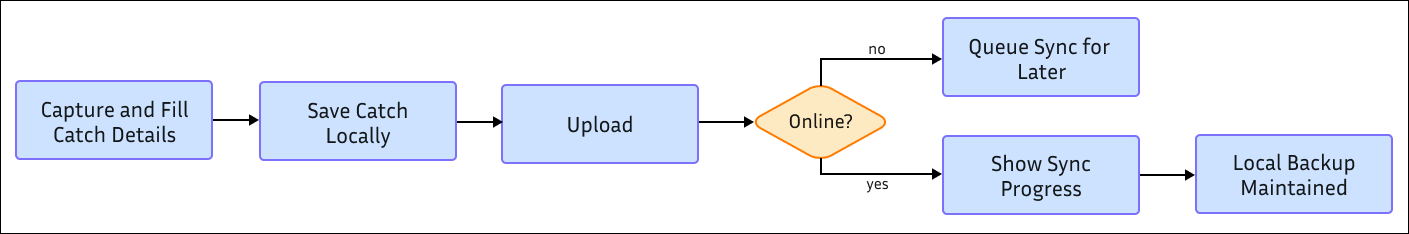
\includegraphics[width=0.45\textwidth]{Landing.png}
    \caption{Returning-to-shore stage use case flow}
    \label{fig:landing}
\end{figure}

\paragraph{Synchronization}
Fig.~\ref{fig:synchronization} shows the synchronization stage. WorkManager evaluates
network and battery constraints and initiates batch upload when conditions are met.
Sessions, catches, violations, GPS tracks, and compressed images (scaled to a maximum
dimension of 1024~px at 70\% JPEG quality) are transmitted to the municipal REST API.
Per-record sync status transitions from PENDING to SYNCED on successful upload or FAILED
on error, with automatic retry scheduled for failed records. The central server
subsequently applies timestamp-based conflict resolution before persisting records to the
aggregated database.

\begin{figure}[h]
    \centering
    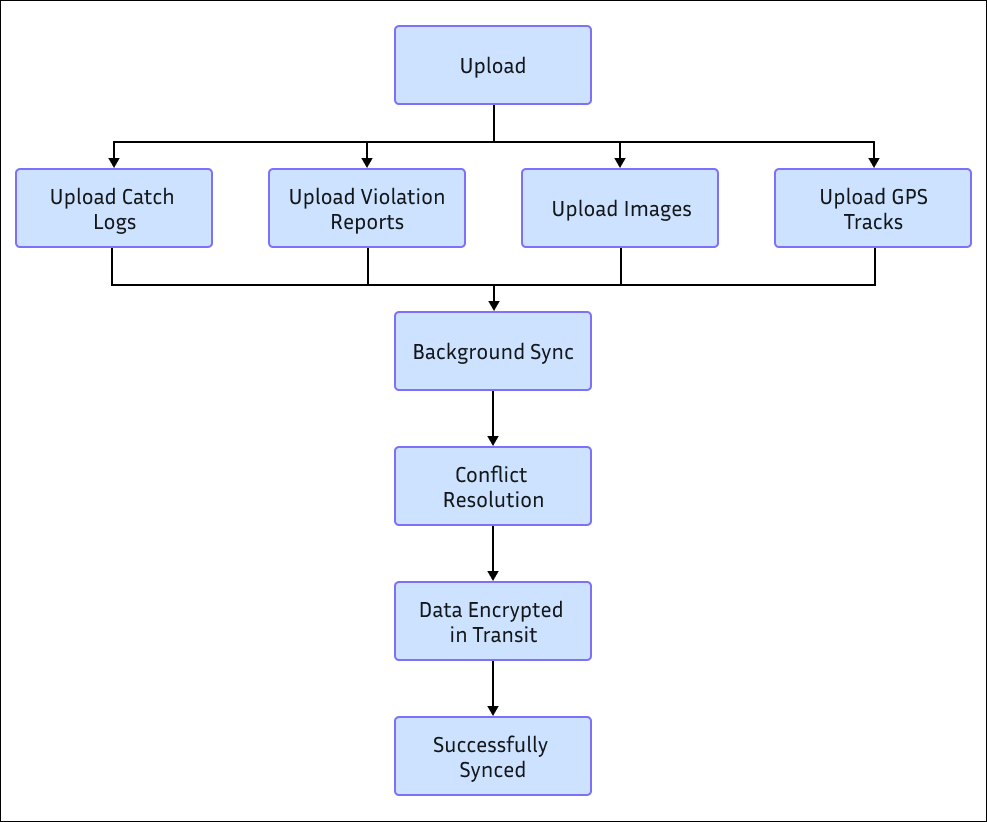
\includegraphics[width=0.45\textwidth]{Synchronization.png}
    \caption{Synchronization stage use case flow}
    \label{fig:synchronization}
\end{figure}

\subsubsection{Web Application Use Case}

The web platform provides three role-differentiated access tiers enforced by JWT
middleware with role-based routing at the API level. The workflows for each role are
illustrated in Figs.~\ref{fig:web_workflow_munic}--\ref{fig:web_workflow_researcher}.

\begin{figure}[h]
    \centering
    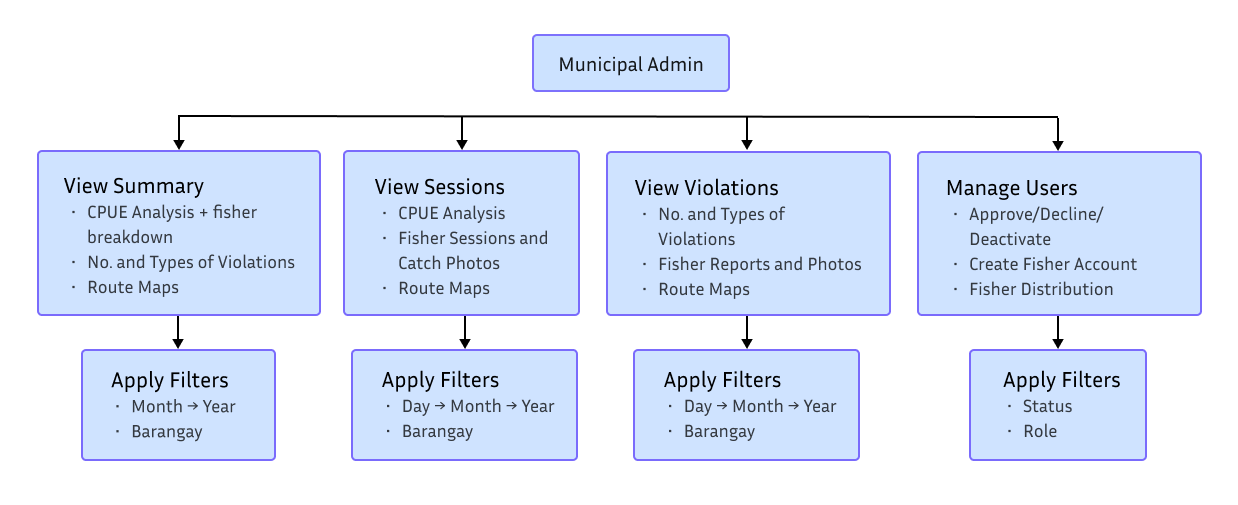
\includegraphics[width=0.45\textwidth]{web_workflow_munic.png}
    \caption{Web Application --- Municipal Administrator Workflow}
    \label{fig:web_workflow_munic}
\end{figure}

\begin{figure}[h]
    \centering
    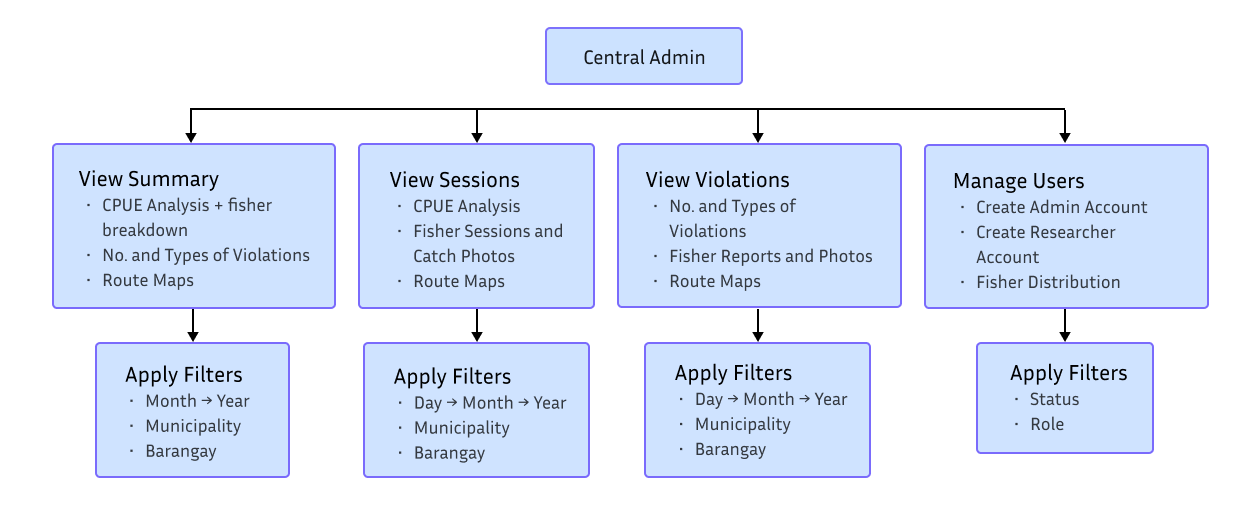
\includegraphics[width=0.45\textwidth]{web_workflow_central.png}
    \caption{Web Application --- Central Administrator Workflow}
    \label{fig:web_workflow_central}
\end{figure}

\begin{figure}[h]
    \centering
    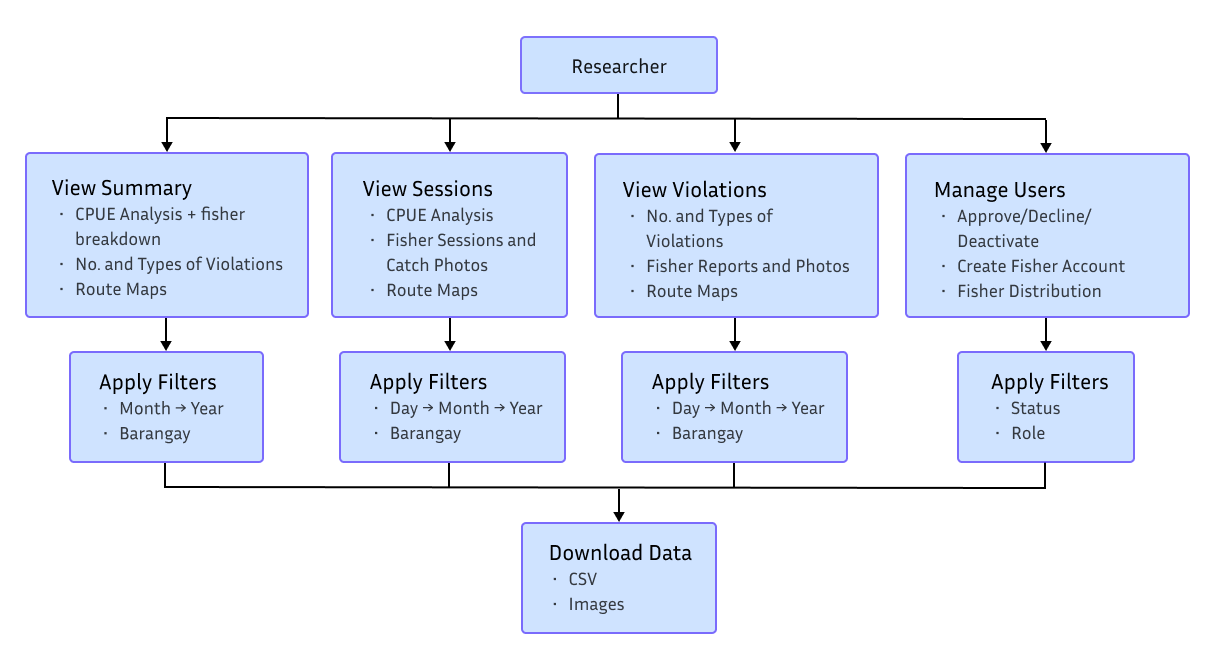
\includegraphics[width=0.45\textwidth]{web_workflow_researcher.png}
    \caption{Web Application --- Researcher Workflow}
    \label{fig:web_workflow_researcher}
\end{figure}

\textbf{Municipal Administrator} (Fig.~\ref{fig:web_workflow_munic}). Approves or
declines fisher registration requests; creates fisher accounts directly; manages user
accounts with municipality assignments; reviews catch logs and violation reports filtered
by date and barangay; views GPS session routes on OpenLayers maps.

\textbf{Central Administrator} (Fig.~\ref{fig:web_workflow_central}). Accesses
aggregated cross-municipality data including CPUE trends, violation pattern summaries,
and session volume statistics. Creates researcher and municipal administrator accounts
from the Manage Users page.

\textbf{Researcher} (Fig.~\ref{fig:web_workflow_researcher}). Views anonymized catch
and violation datasets with filtering by date, municipality, and barangay. Accesses CPUE
aggregates, species distribution data, and fisher registration statistics for conservation
trend analysis without exposure to individual fisher identities. Downloads CSV and image
exports from all four dashboard tabs.

\subsection{Evaluation: System Usability Scale (SUS)}

Usability evaluation was conducted using the System Usability Scale (SUS), a validated
10-item questionnaire producing scores on a 0--100 scale. Scores above 68 are considered
above average; scores above 80.3 are rated excellent \cite{Bangor2008}. Evaluation was
conducted separately for three system components---the mobile application, the municipal
administrator dashboard, and the researcher dashboard---with five respondents assigned to
each (15 total). Respondents were general users tasked with completing representative
workflows on their assigned platform. No domain background in fisheries was required,
reflecting the system's design goal of accessibility across varying digital literacy
levels. SUS items were rated immediately following guided task interaction sessions.

%% ============================================================
%% SECTION IV — RESULTS AND DISCUSSION
%% ============================================================

\section{Results and Discussion}

The development of BantayLaot+ produced a functional,
multi-component fisheries monitoring system consisting of an Android mobile application,
two municipality-level REST API servers, a central cloud-hosted aggregation server, and a
role-differentiated web platform, intended for deployment across two municipalities in
Misamis Oriental. All primary objectives stated in the study were achieved: the mobile
application supports offline-first operation with background synchronization; and the web
platform delivers structured multi-role data access. The structured image pipeline
established during development provides the dataset infrastructure required for future
AI model training once field deployment is initiated.

\subsection{Mobile Application}

The mobile application was implemented in Kotlin using traditional Android Views with
View Binding and tested on Android devices during development. The interface is organized around a
session-based workflow guiding fisherfolk sequentially through pre-departure preparation,
at-sea operations, catch documentation, and synchronization. The following subsections
present the key interface views produced during development.

\subsubsection{Authentication and Session Initialization}

\begin{figure}[h]
    \centering
    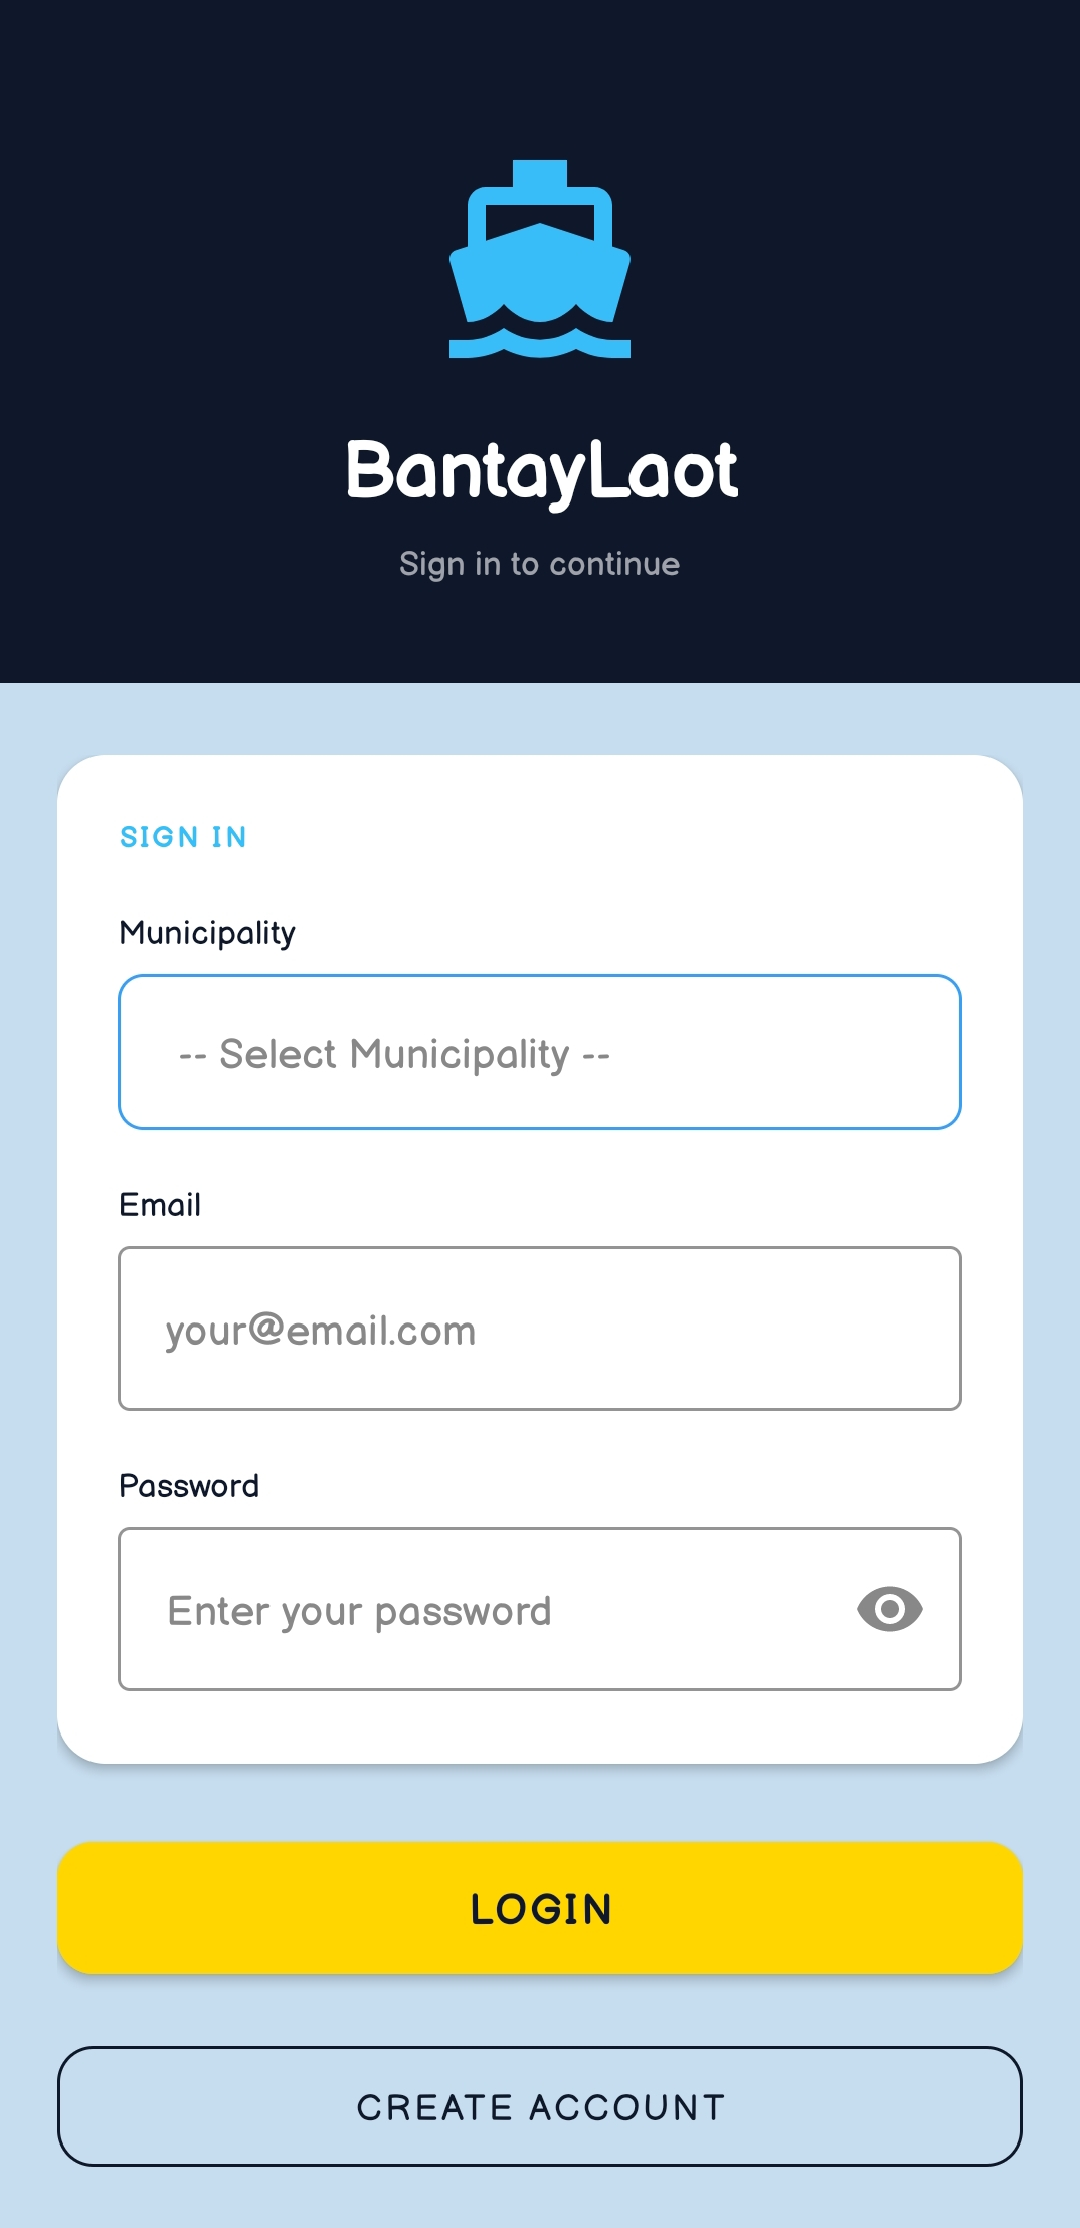
\includegraphics[width=0.3\textwidth]{mobile_login.jpg}
    \caption{Mobile Application --- Login Screen}
    \label{fig:mobile_login}
\end{figure}

\begin{figure}[h]
    \centering
    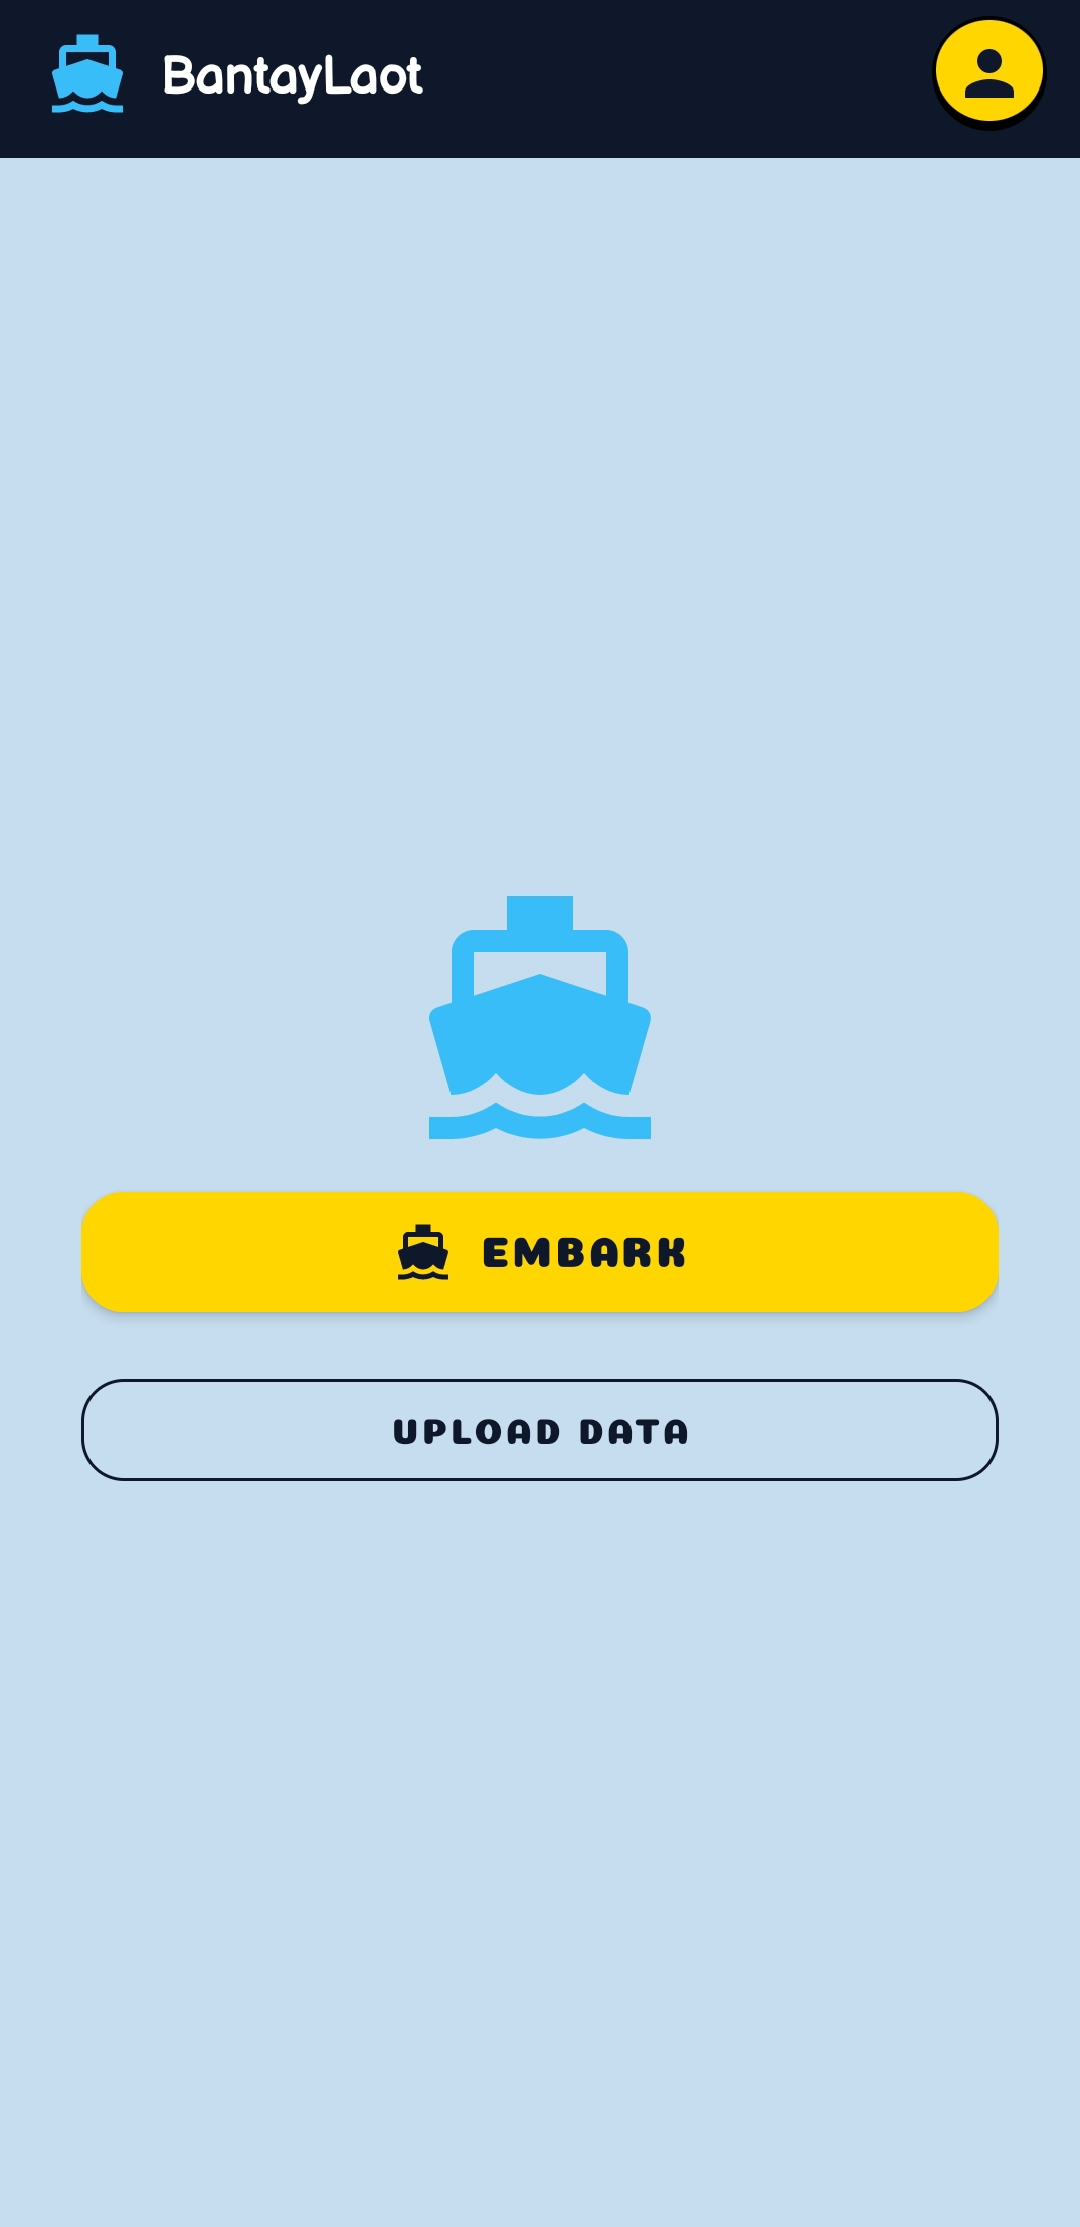
\includegraphics[width=0.3\textwidth]{mobile_home.jpg}
    \caption{Mobile Application --- Home Dashboard}
    \label{fig:mobile_home}
\end{figure}

Upon launching the application, fisherfolk authenticate using credentials issued by the
municipal administrator, as shown in Fig.~\ref{fig:mobile_login}. JWT tokens received
upon successful login are persisted in SharedPreferences, allowing the application to
remain accessible offline without requiring repeated server authentication for subsequent
sessions. Upon authentication, the user is directed to the home dashboard
(Fig.~\ref{fig:mobile_home}), which presents the current session status and provides
access to all primary functions: starting a new fishing session, reporting violations,
documenting catches, and uploading data to the server.

\subsubsection{Pre-Departure and GPS Initialization}

\begin{figure}[h]
    \centering
    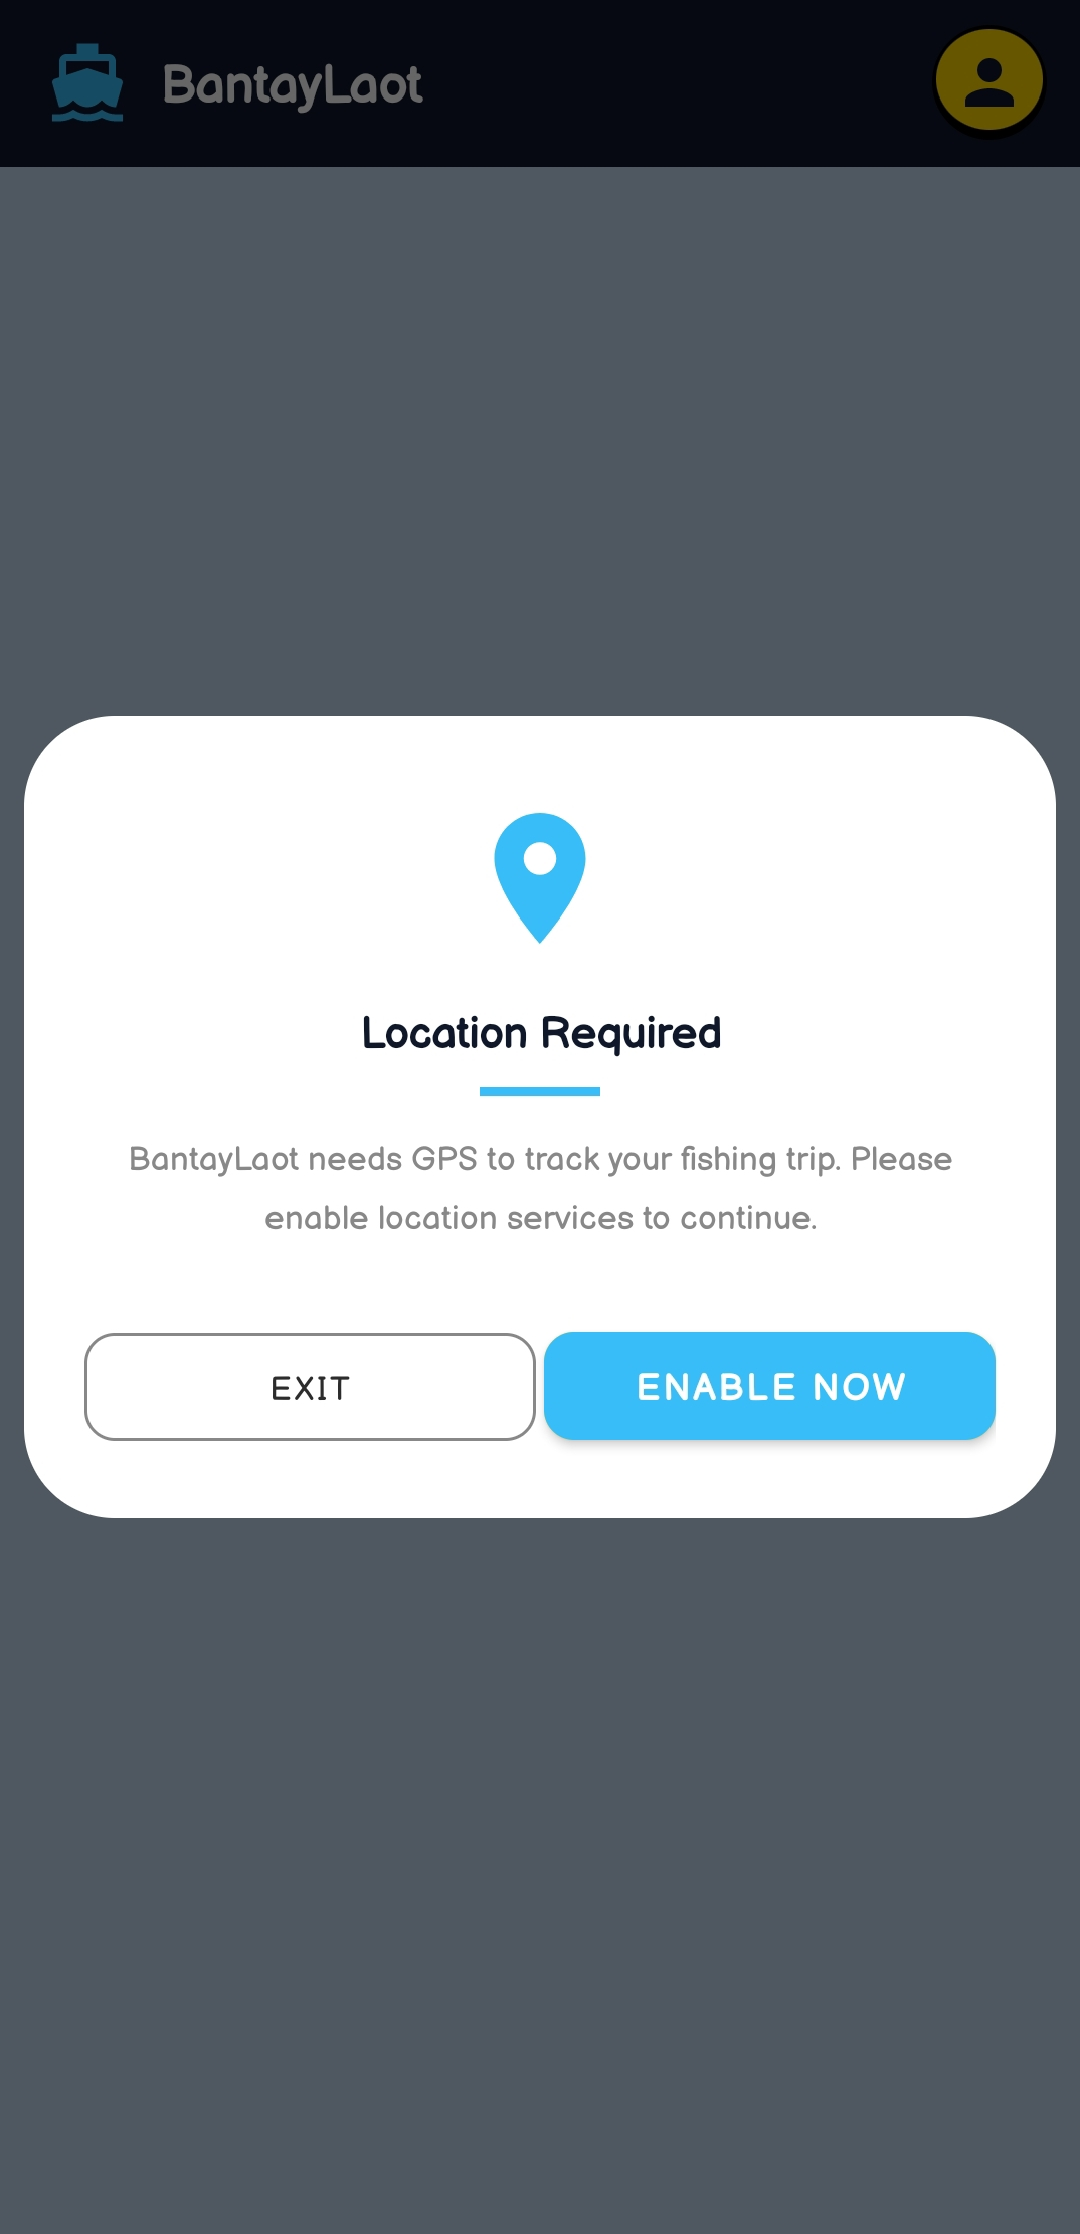
\includegraphics[width=0.3\textwidth]{mobile_predeparture.jpg}
    \caption{Mobile Application --- Pre-Departure Session Start}
    \label{fig:mobile_predeparture}
\end{figure}

As illustrated in Fig.~\ref{fig:mobile_predeparture}, when initiating a session, the
application verifies location permissions and begins recording GPS coordinates via Android
Location Services. An active session indicator confirms that GPS tracking is running in
the background. All session metadata---start timestamp, fisher identifier, and municipality
assignment---is written to Room Database immediately upon session creation, decoupled from
server availability.

\subsubsection{At-Sea Operations and Violation Reporting}

\begin{figure}[h]
    \centering
    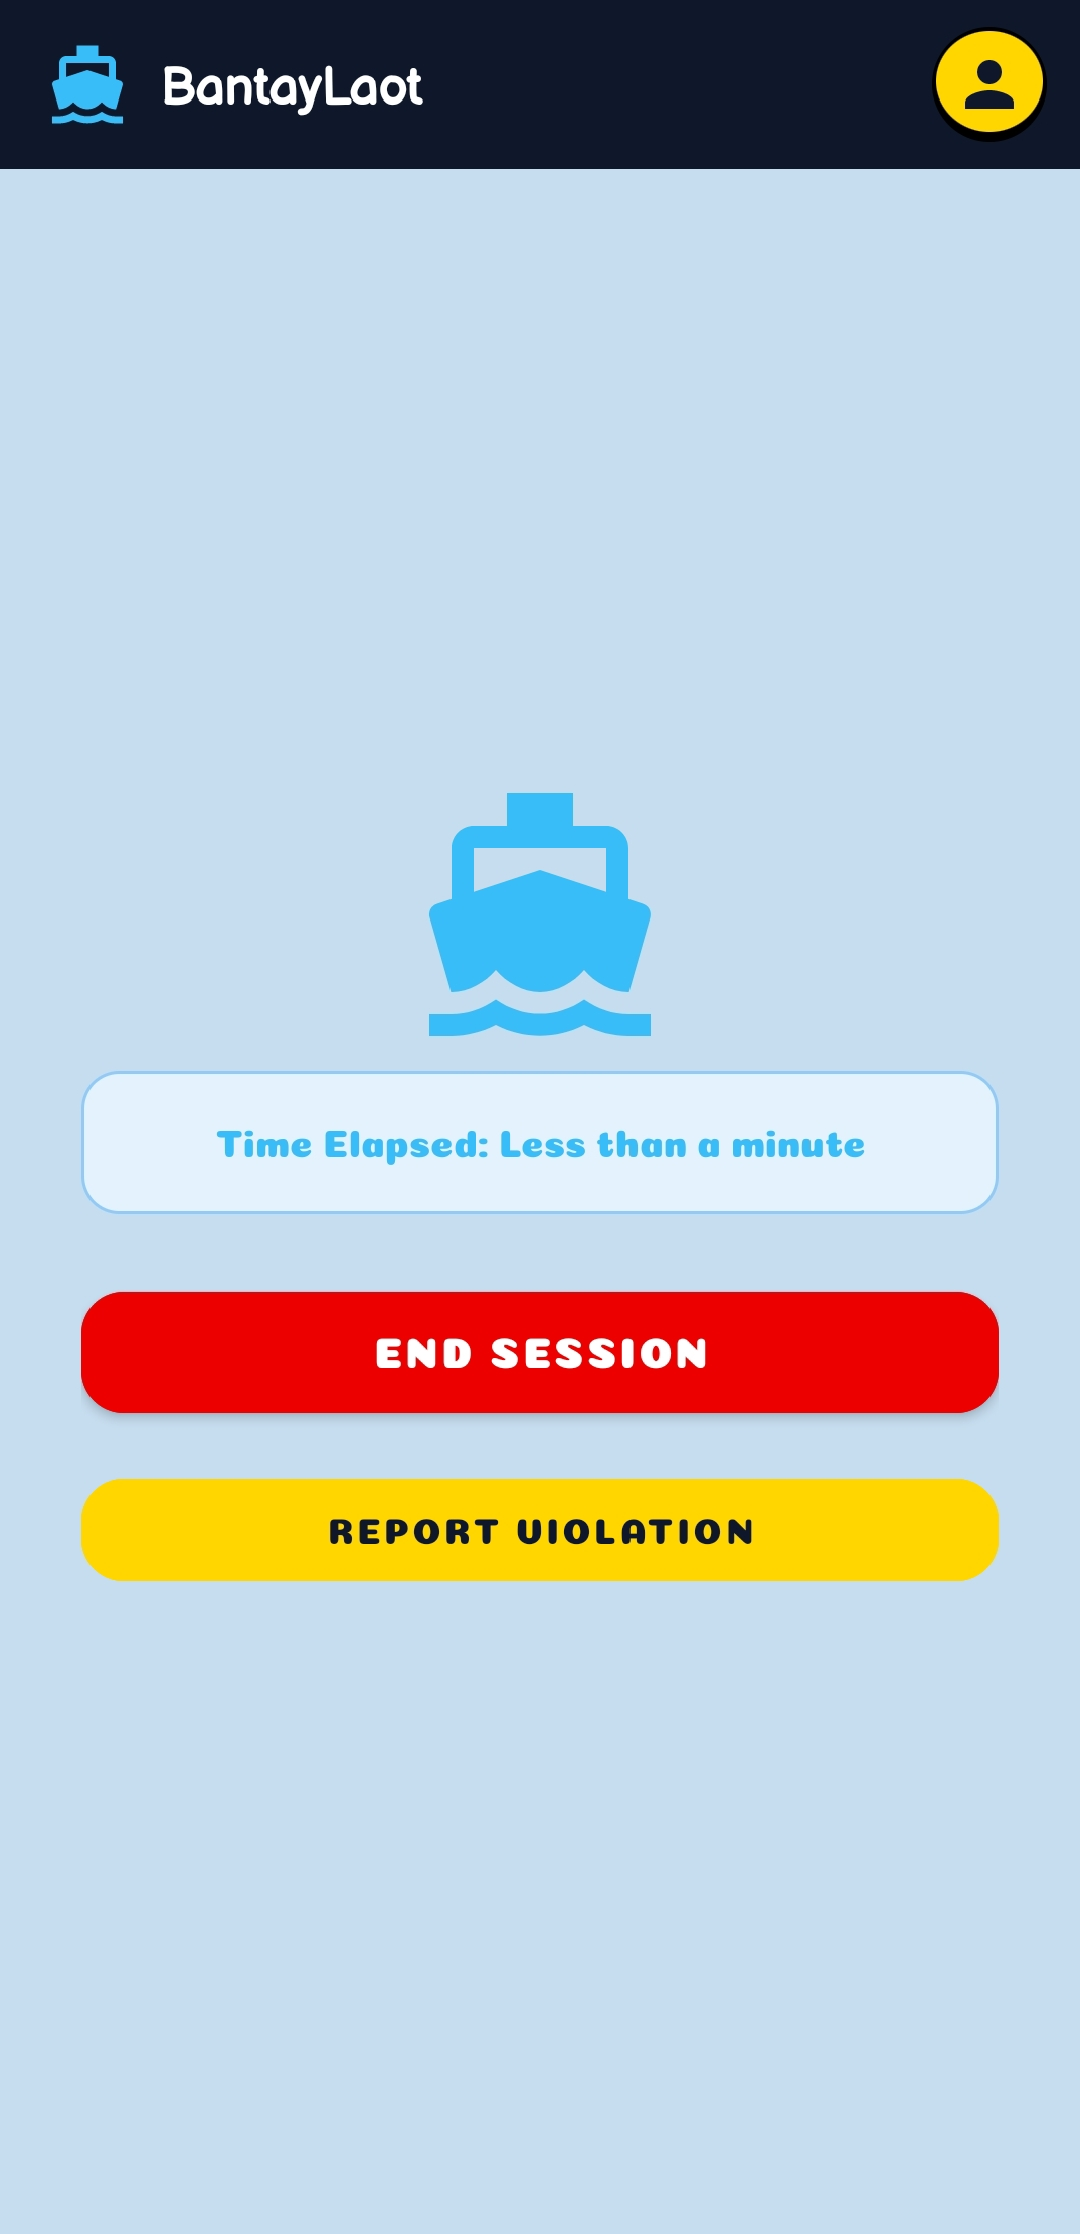
\includegraphics[width=0.3\textwidth]{mobile_atsea.jpg}
    \caption{Mobile Application --- Active Fishing Session View (At Sea)}
    \label{fig:mobile_atsea}
\end{figure}

\begin{figure}[h]
    \centering
    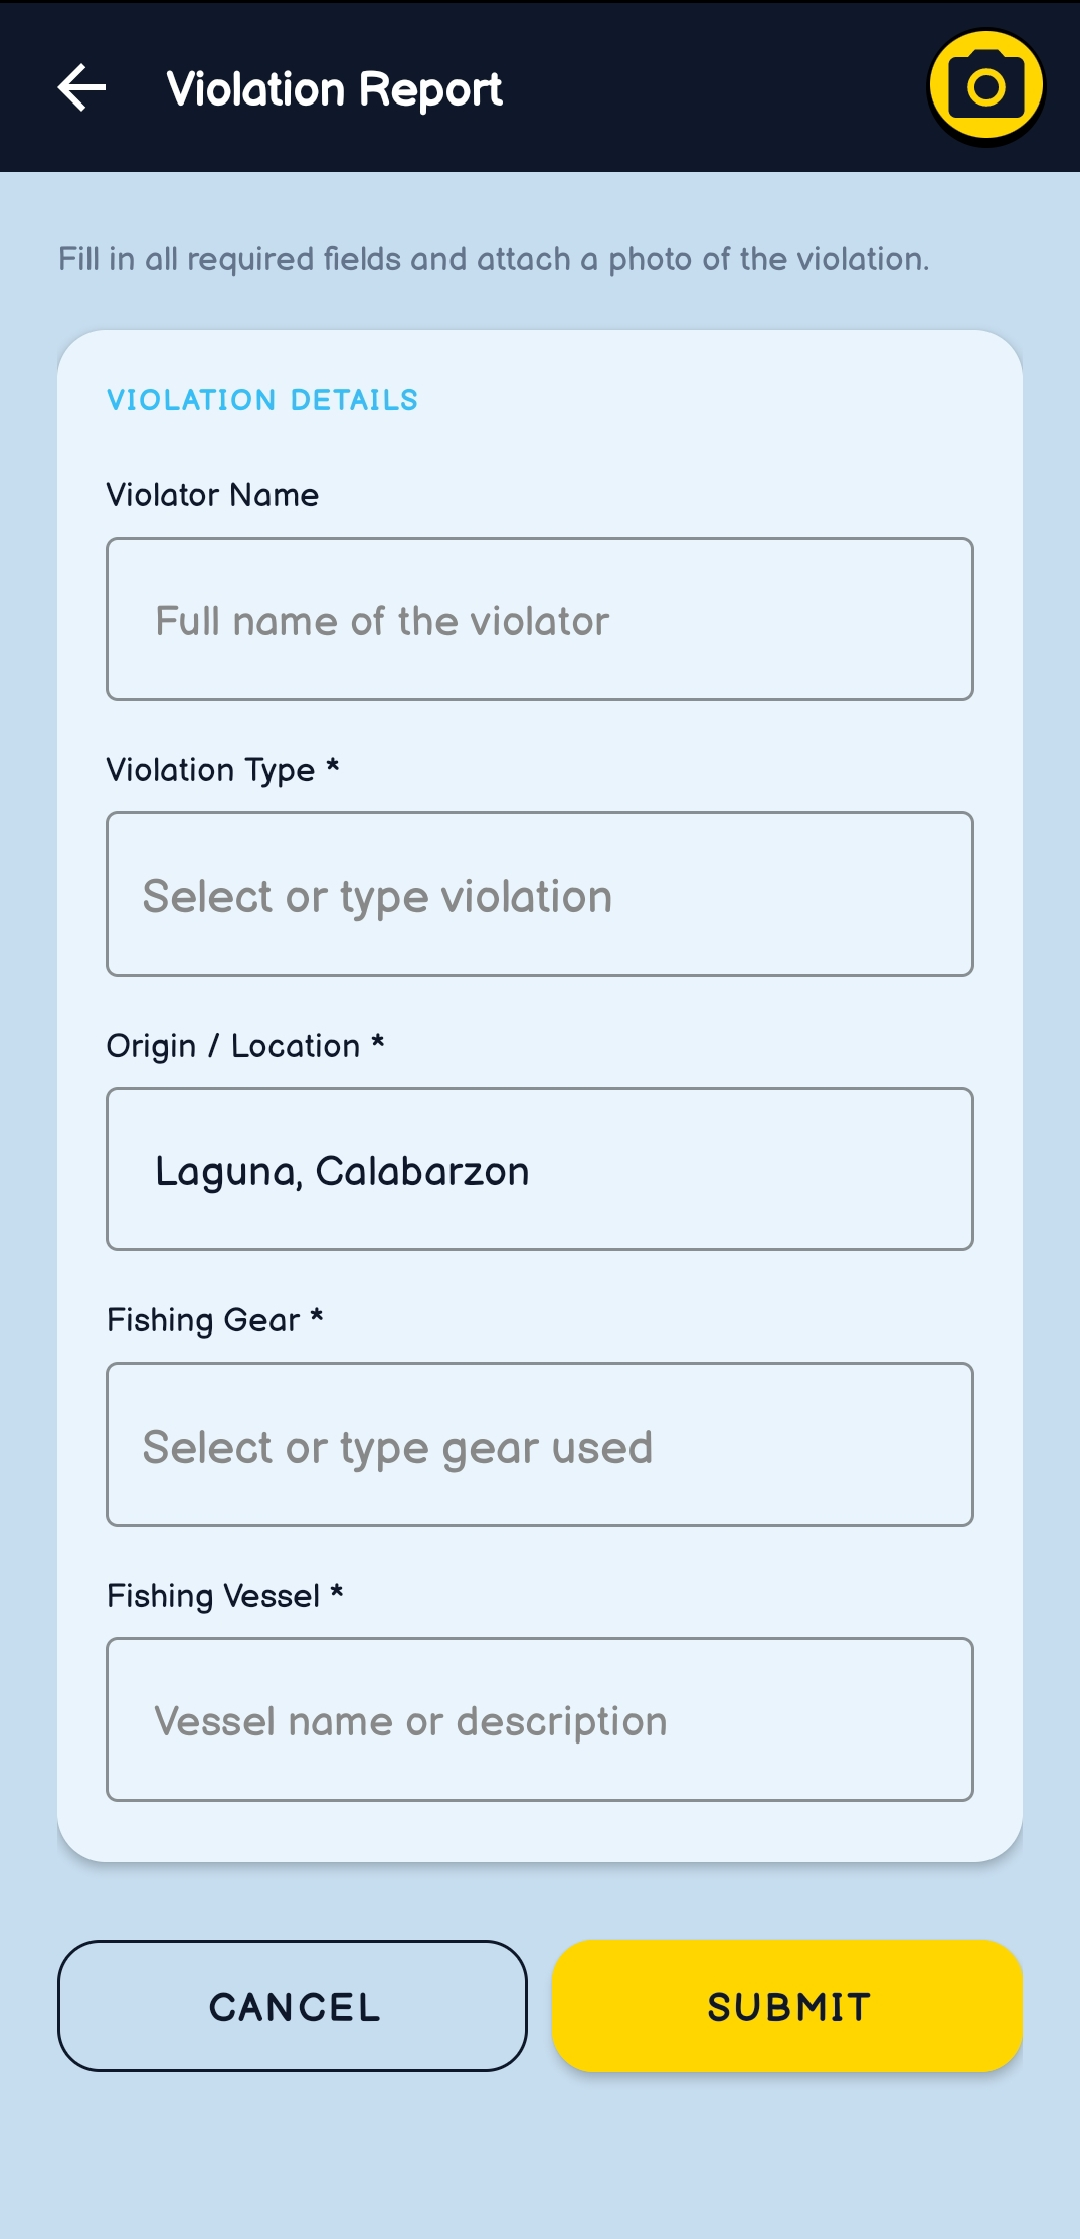
\includegraphics[width=0.3\textwidth]{mobile_violation.jpg}
    \caption{Mobile Application --- Violation Reporting Form}
    \label{fig:mobile_violation}
\end{figure}

Fig.~\ref{fig:mobile_atsea} shows the active session view displayed during at-sea
operations. GPS fixes are recorded every 30 seconds to Room Database regardless of
network state. When a violation is observed, the fisherfolk accesses the violation
reporting form shown in Fig.~\ref{fig:mobile_violation}, which allows capture of a
geotagged photograph and manual entry of the violating vessel description, gear type, and
narrative notes. Geographic coordinates at the time of submission are automatically
attached to the violation record, and the report is stored locally with PENDING status
and queued for upload.

\subsubsection{Catch Documentation}

\begin{figure}[h]
    \centering
    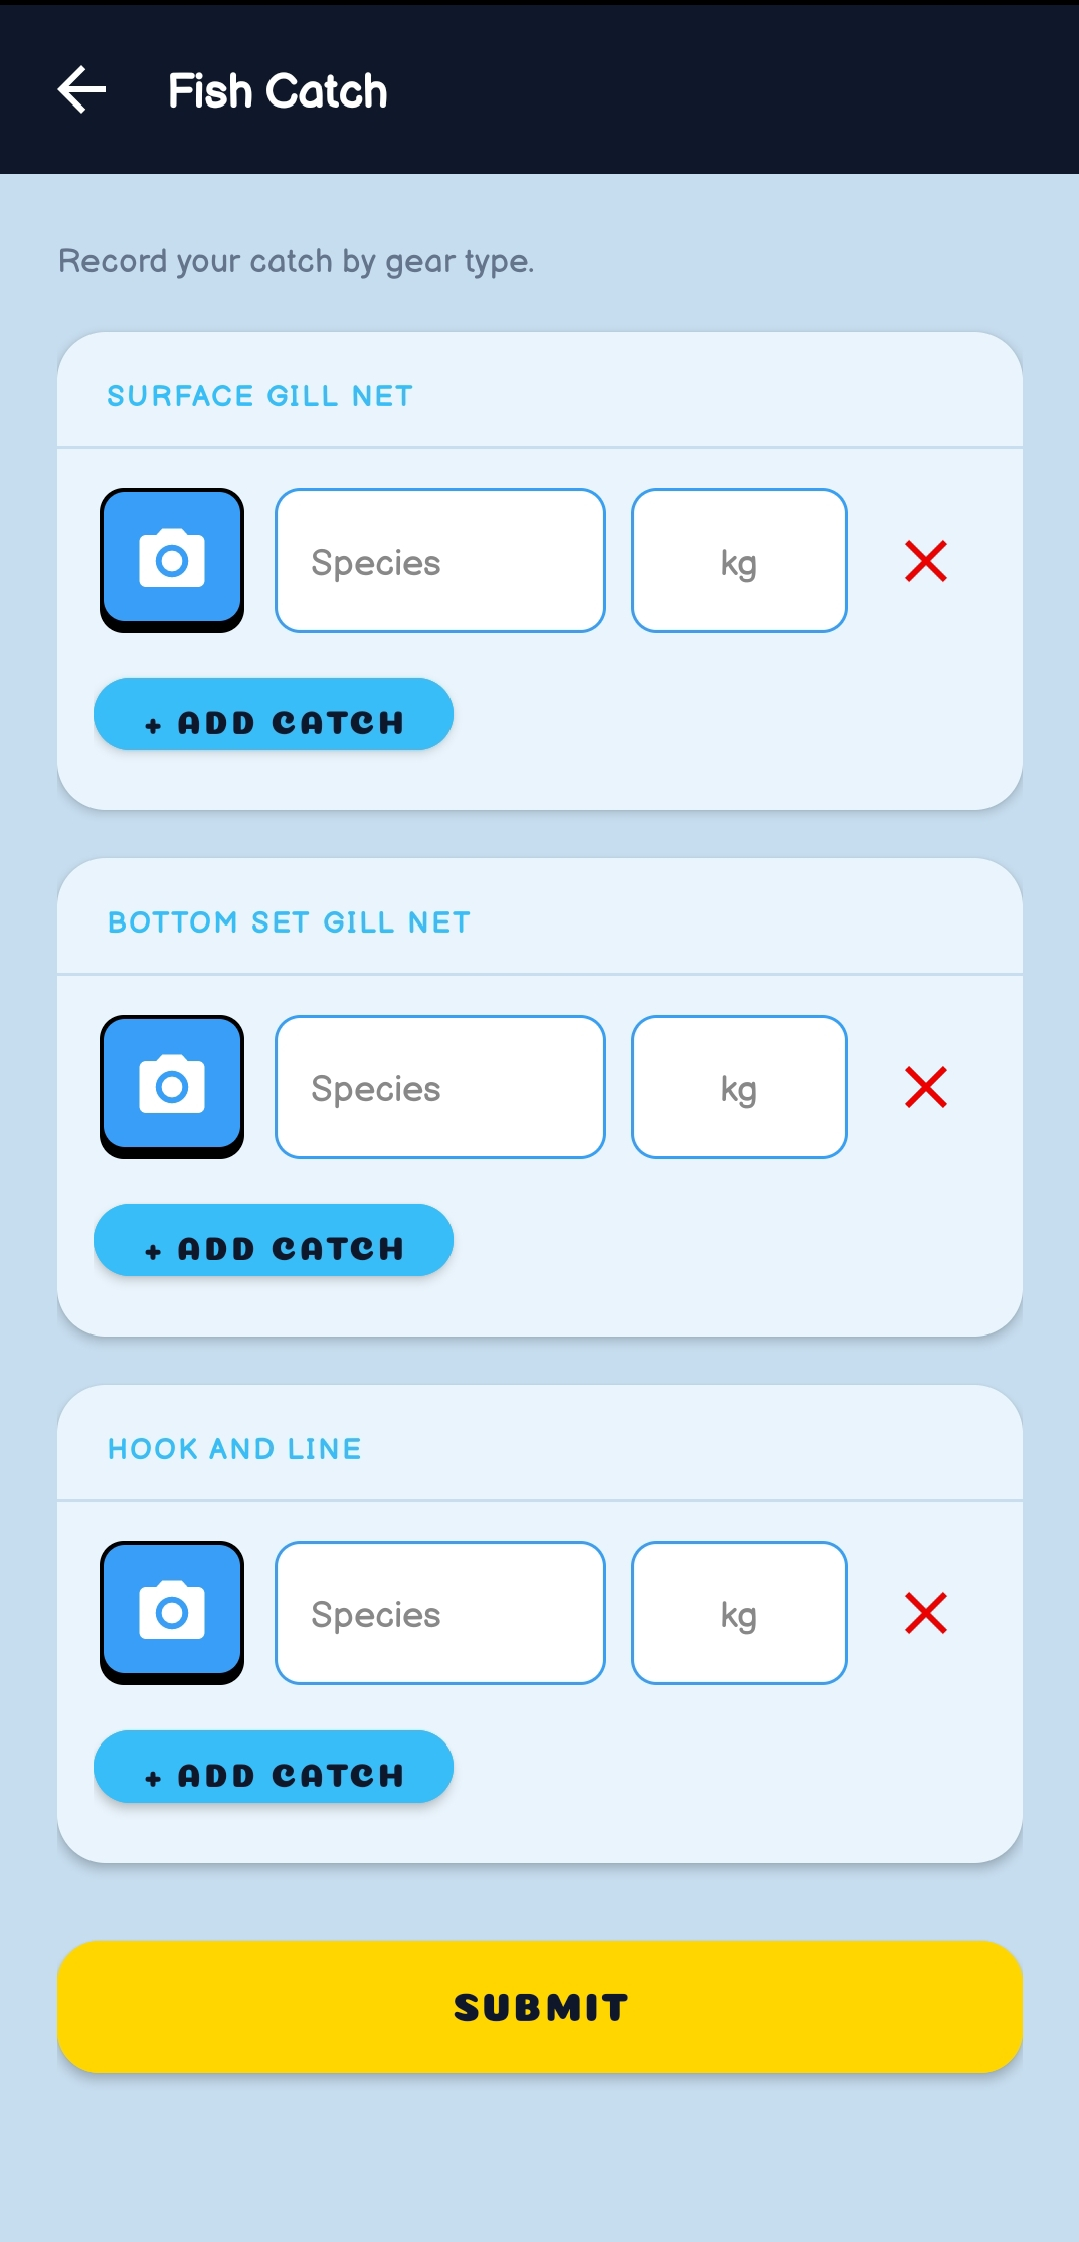
\includegraphics[width=0.3\textwidth]{mobile_catch.jpg}
    \caption{Mobile Application --- Catch Documentation}
    \label{fig:mobile_catch}
\end{figure}

Catch documentation is initiated upon returning to shore. As shown in
Fig.~\ref{fig:mobile_catch}, the fisherfolk captures a photograph of each haul and then
enters catch details manually. The species and weight entry form allows the fisherfolk to select a species from an
autocomplete dropdown of 975 recognized Philippine species, enter weight in kilograms,
and select one of three gear categories: Surface Gill Net, Bottom Set Gill Net, or Hook
and Line. The underlying data model is structured so that a future AI classification
backend can be integrated without schema changes.

\subsubsection{Upload and Synchronization}

Synchronization is initiated from the home screen via a visible Upload button, which is
accessible when no session is active. Tapping the button reinitializes the Retrofit client
with the latest stored token and enqueues a one-time WorkManager task constrained to any
active network connection. The home screen observes the WorkManager status and provides
inline toast feedback: a queued state when awaiting connectivity, a running state during
active upload, and success or failure states upon completion. Failed uploads are
automatically retried by the periodic WorkManager task, which runs approximately every
hour. Per-entity sync states (PENDING, SYNCED, FAILED) are tracked in Room Database for
sessions, catches, violations, and GPS tracks, ensuring no record is retransmitted
unnecessarily.

\subsection{Web Application}

The web application was developed using React.js. Three distinct
dashboard views were implemented for municipal administrators, central administrators, and
researchers, each enforced by JWT middleware with role-based routing at the API level.

\subsubsection{Municipal Administrator Dashboard}

\begin{figure}[h]
    \centering
    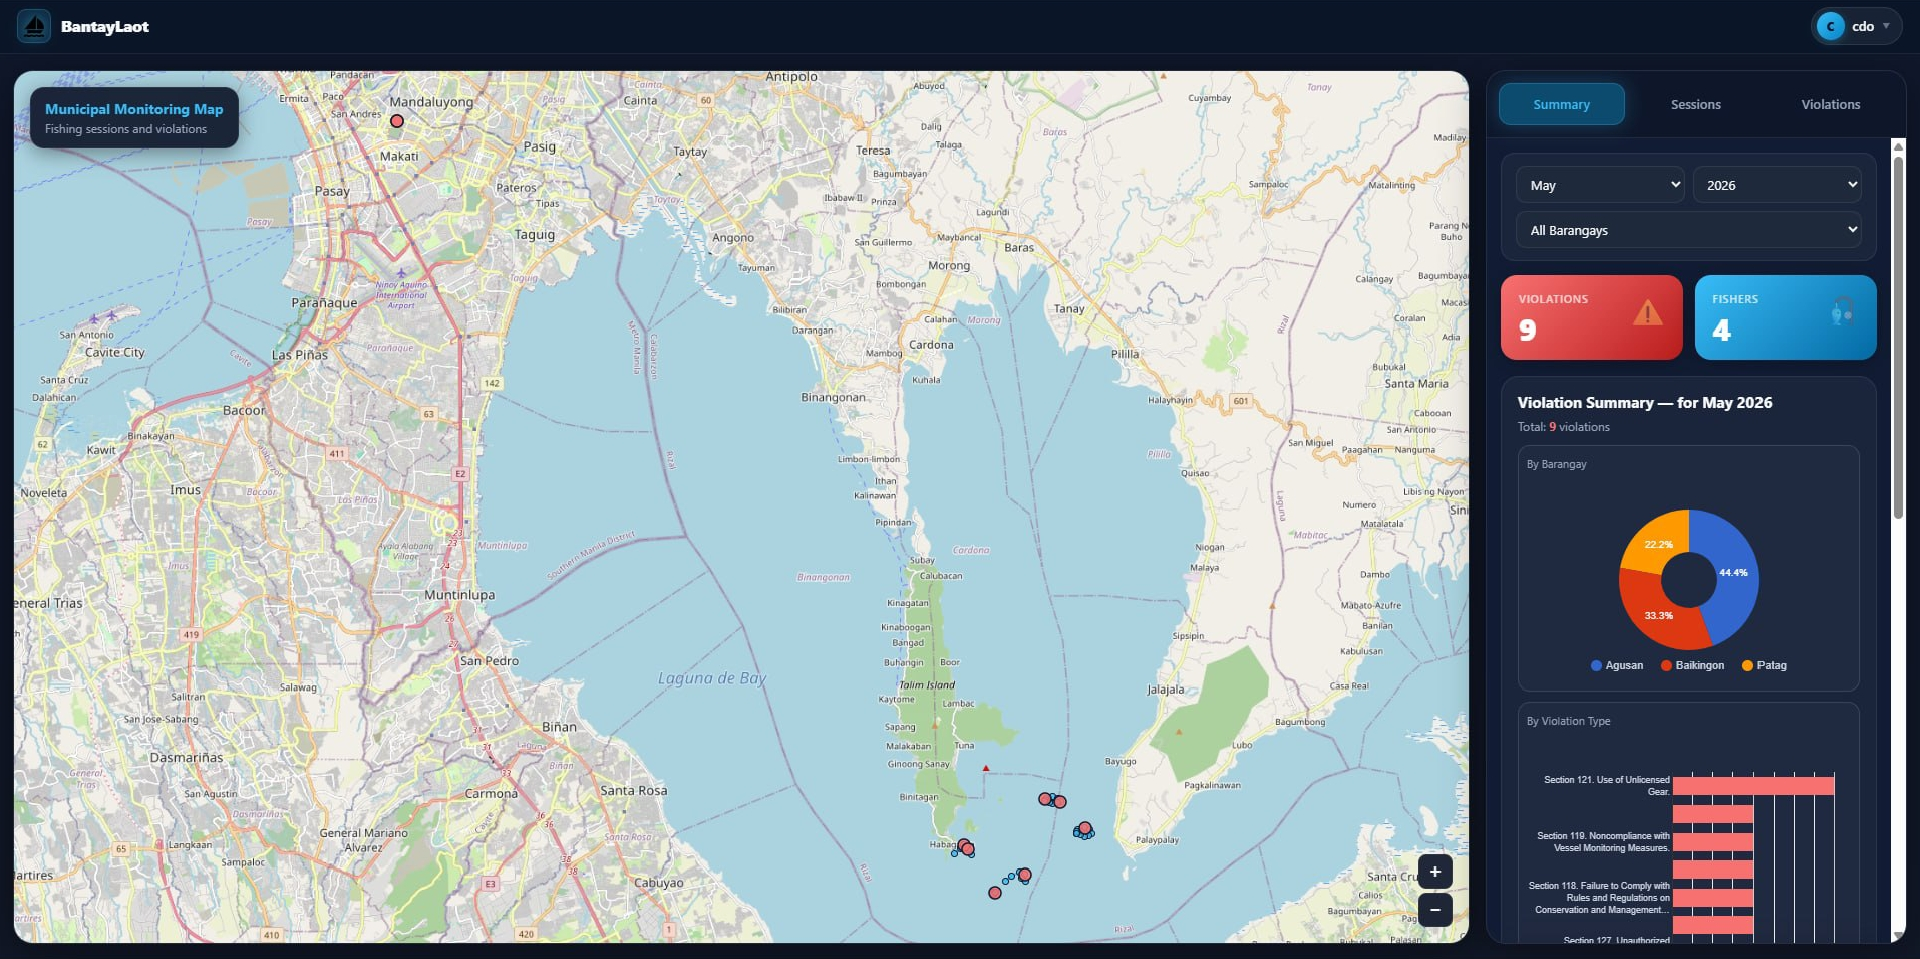
\includegraphics[width=0.45\textwidth]{web_munic_overview.jpg}
    \caption{Web Application --- Municipal Administrator Summary Tab}
    \label{fig:web_munic_overview}
\end{figure}

\begin{figure}[h]
    \centering
    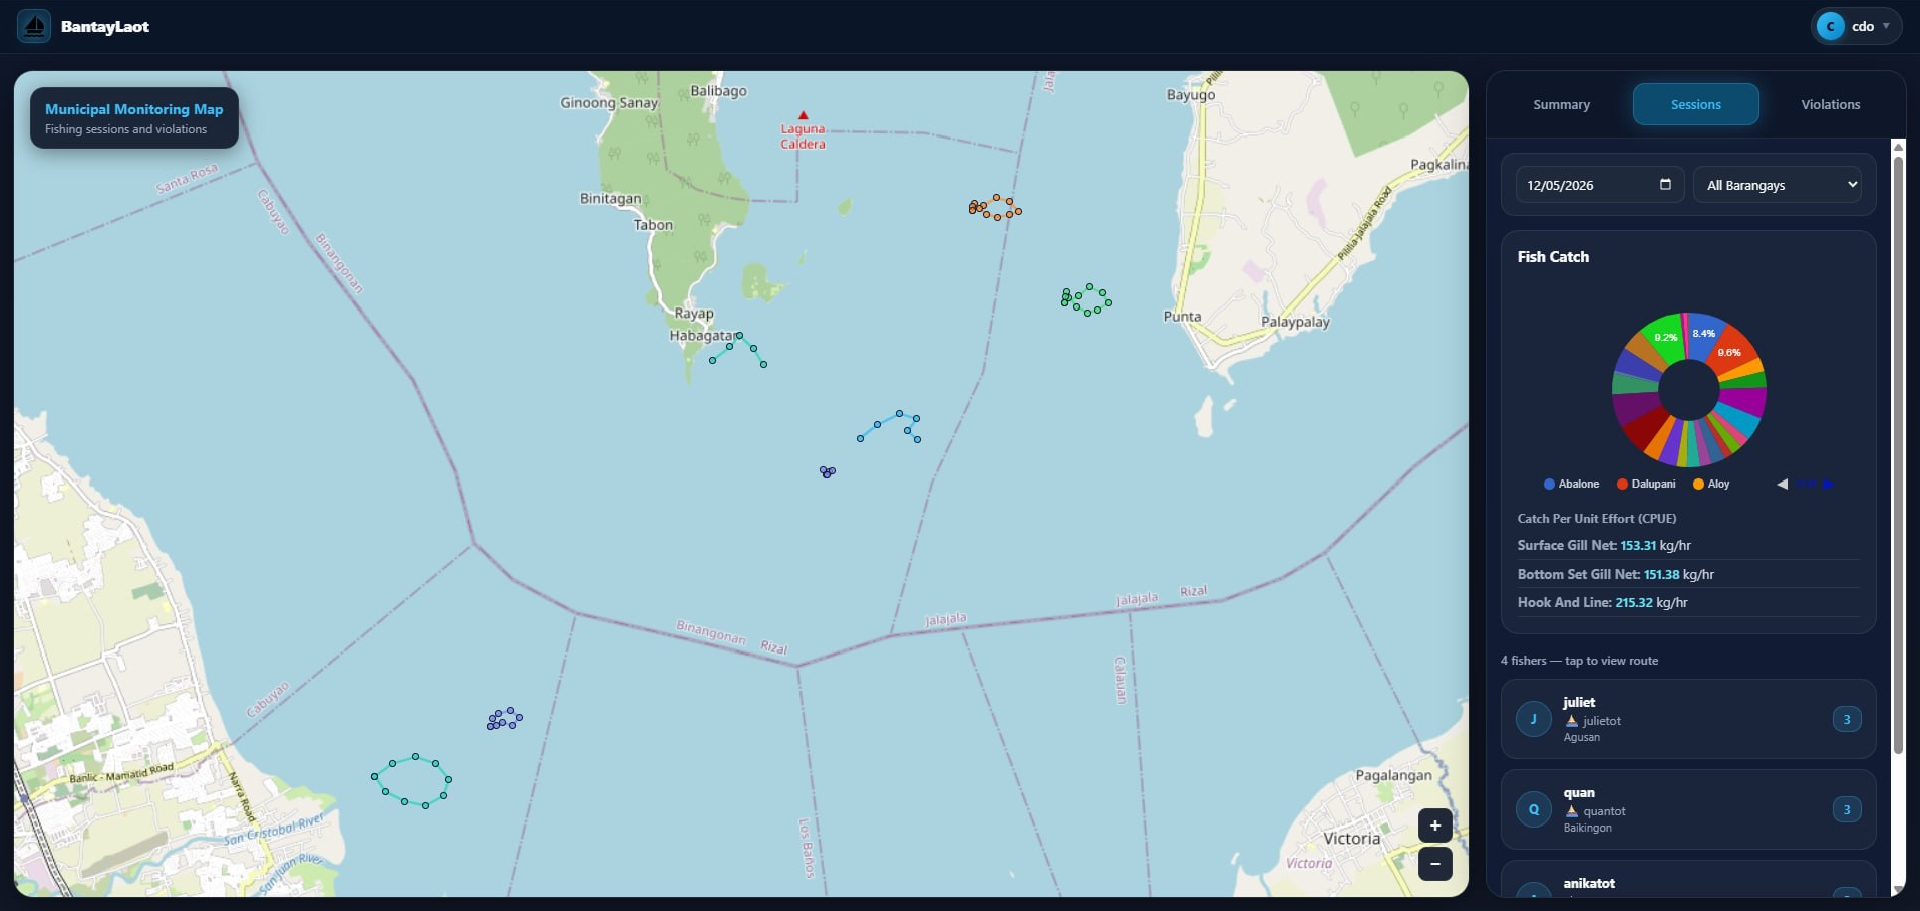
\includegraphics[width=0.45\textwidth]{web_munic_sessions.jpg}
    \caption{Web Application --- Sessions Tab with Expanded Fisher Detail (Municipal View)}
    \label{fig:web_munic_sessions}
\end{figure}

\begin{figure}[h]
    \centering
    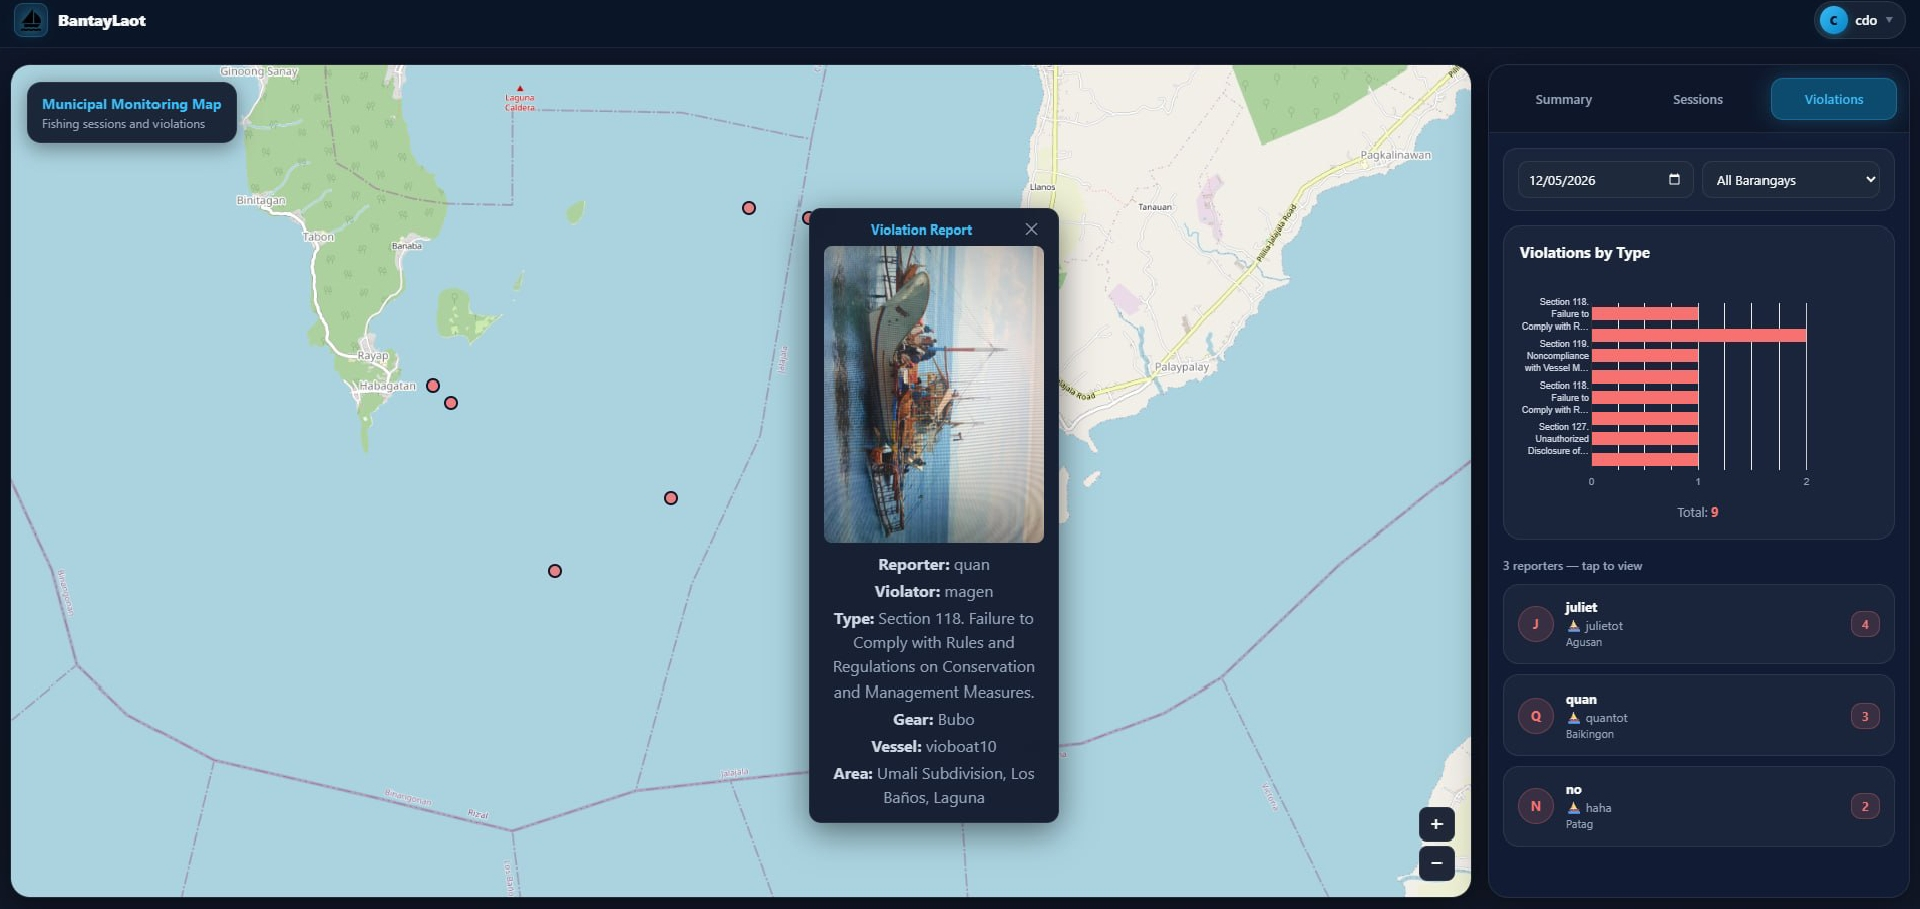
\includegraphics[width=0.45\textwidth]{web_munic_violations.jpg}
    \caption{Web Application --- Violations Tab with Expanded Violation Detail (Municipal View)}
    \label{fig:web_munic_violations}
\end{figure}

\begin{figure}[h]
    \centering
    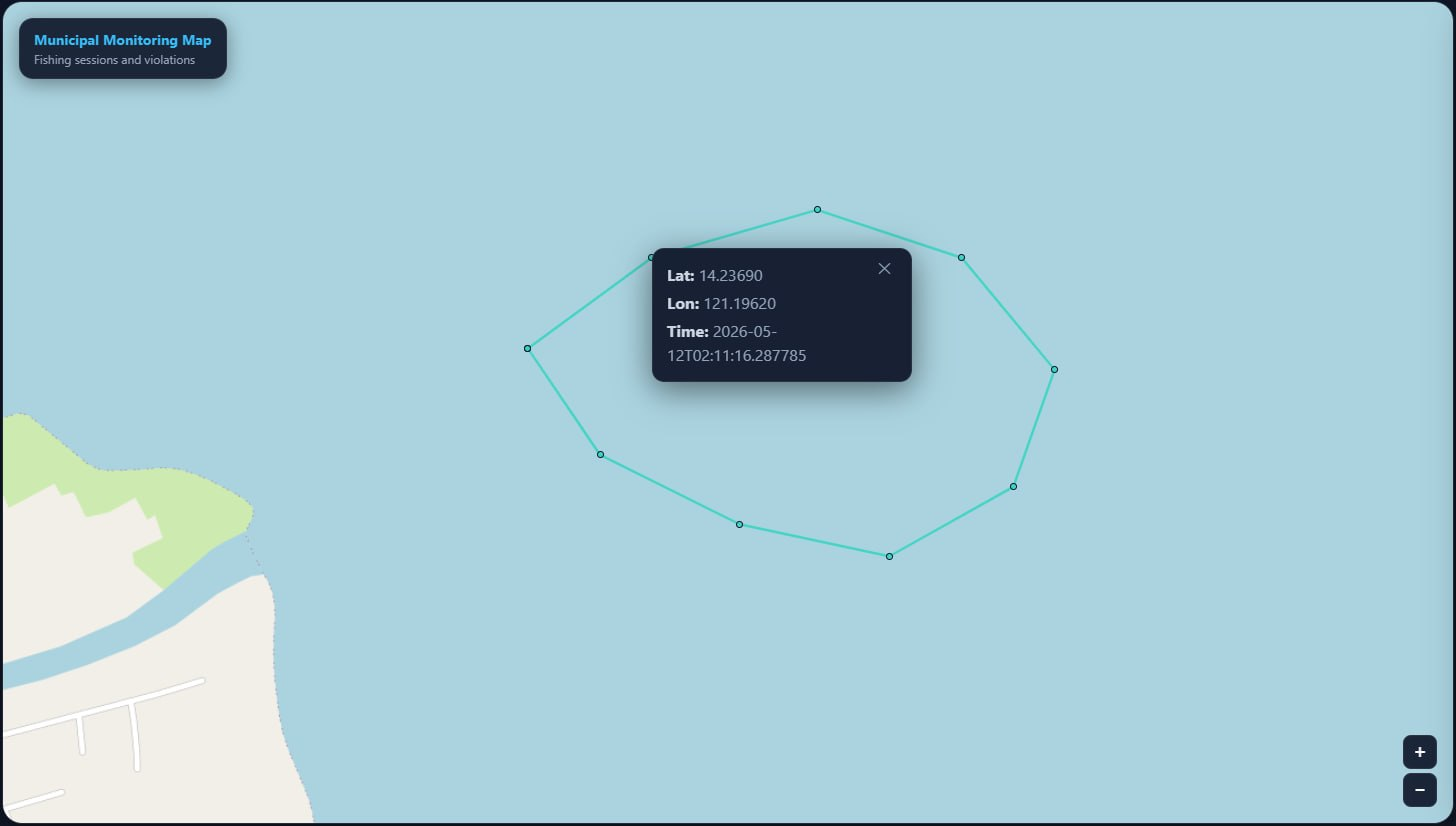
\includegraphics[width=0.45\textwidth]{web_munic_map.jpg}
    \caption{Web Application --- GPS Session Route Rendered as OpenLayers Polyline
             (Municipal View)}
    \label{fig:web_munic_map}
\end{figure}

\begin{figure}[h]
    \centering
    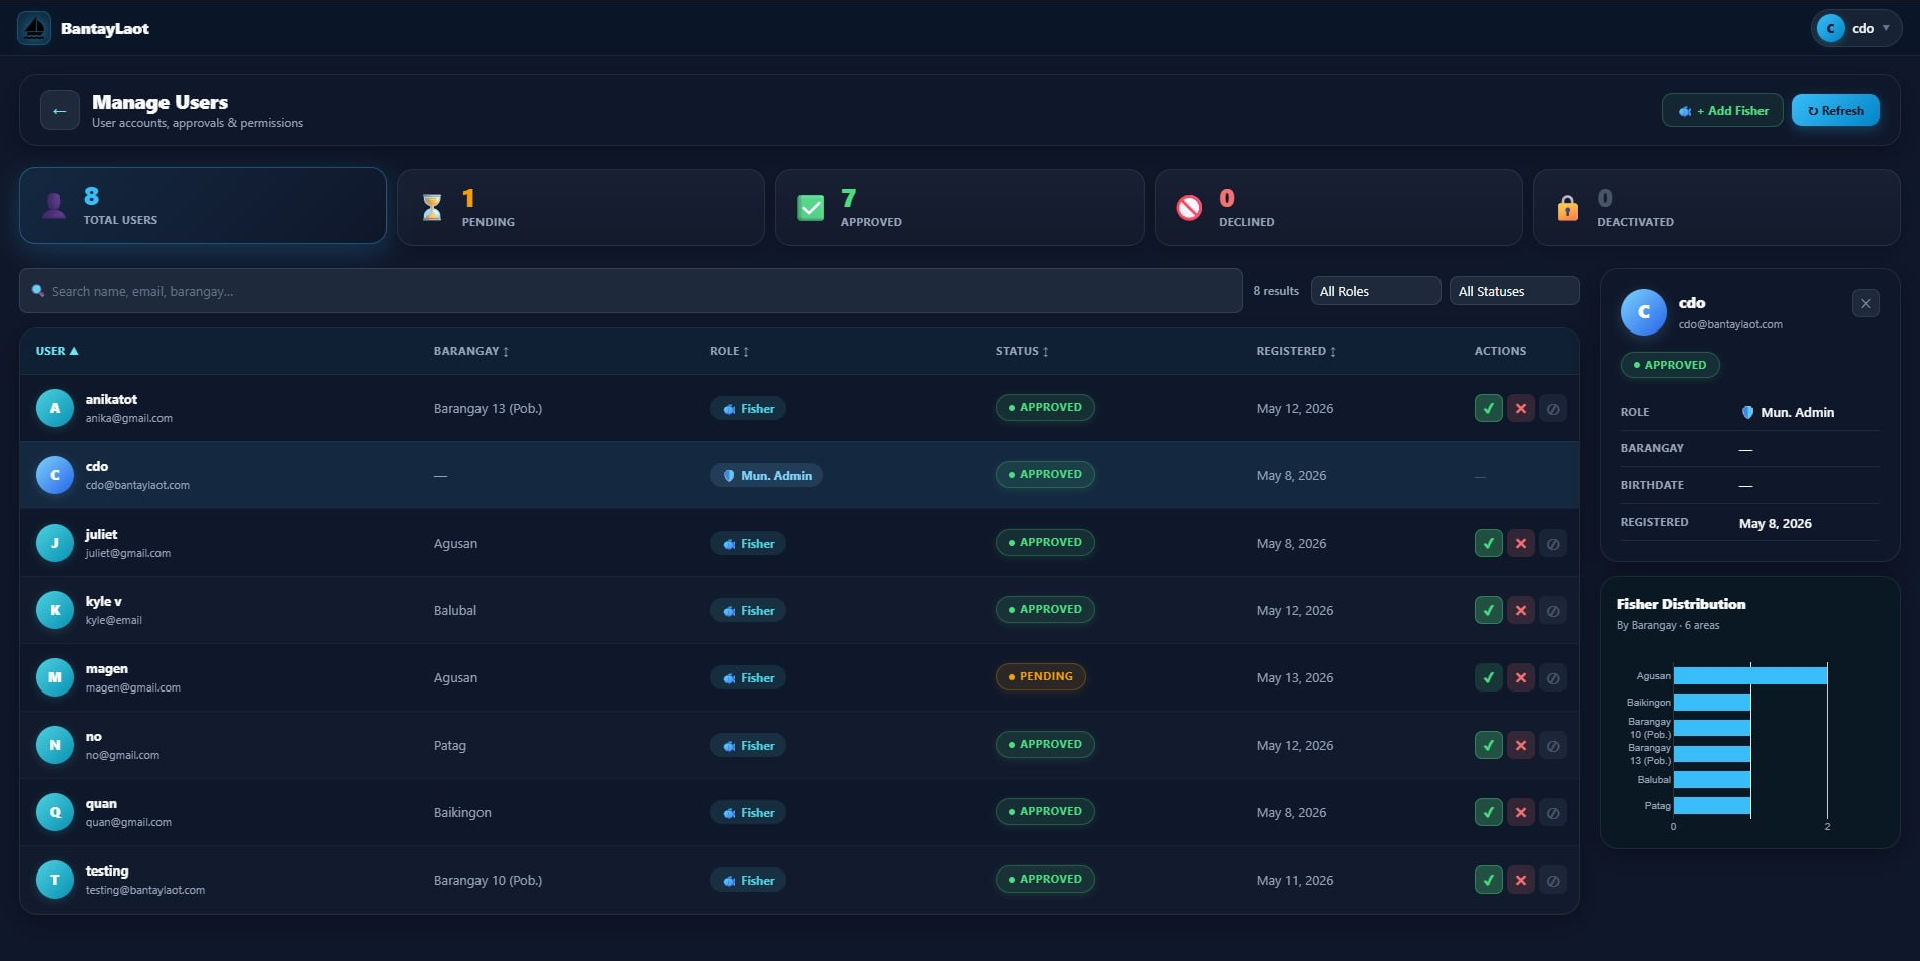
\includegraphics[width=0.45\textwidth]{web_munic_users.jpg}
    \caption{Web Application --- Manage Users Page (Municipal View)}
    \label{fig:web_munic_users}
\end{figure}

The municipal administrator dashboard, shown in Fig.~\ref{fig:web_munic_overview},
provides jurisdiction-level operational oversight through three tabs. The Summary Tab
offers month, year, and barangay filters and displays two stat cards---total violations
and active fishers for the selected period. Below the stat cards, a Violation Summary
card presents a Google Charts pie chart of violations by barangay and a bar chart grouped
by violation type. A CPUE card follows, showing a fish species catch pie chart, a
per-gear CPUE row expressing catch in kilograms per hour, and an expandable fisher
breakdown with session counts per fisher.

The Sessions Tab, illustrated in Fig.~\ref{fig:web_munic_sessions}, is filtered by a
single date input and an optional barangay selector. It opens with a daily fish catch
pie chart and a CPUE summary row, followed by a list of fisher cards each bearing a
session count badge. Selecting a fisher card expands a detail view containing the
session's start and end timestamps, a catch analysis pie chart, per-gear CPUE values,
and catch photographs retrieved from Cloudinary. The GPS route recorded during that
session is rendered as an OpenLayers polyline on the map shown in
Fig.~\ref{fig:web_munic_map}, providing a spatial record of the vessel's path within
the municipality.

The Violations Tab (Fig.~\ref{fig:web_munic_violations}) shares the same date and
barangay filters. A bar chart of violations by type appears at the top with a running
total, followed by reporter cards. Expanding a card reveals the violation photograph,
the violator's identity, the specific violation type, the fishing gear and vessel
involved, the reported origin area, and the submission timestamp.

User registration management is handled through a separate Manage Users page
(Fig.~\ref{fig:web_munic_users}). The page presents a sortable table of all accounts
registered within the municipality, with role badges distinguishing Fishers, Municipal
Admins, and Researchers, and status badges indicating whether each account is Approved,
Pending, Declined, or Deactivated. Municipal administrators review incoming registration
requests and approve, decline, or deactivate accounts directly from this interface.
They may also bypass the self-registration flow entirely by using the Add Fisher form,
which creates a fisher account pre-approved with full boat and location details supplied
at creation time.

\subsubsection{Central Administrator Dashboard}

\begin{figure}[h]
    \centering
    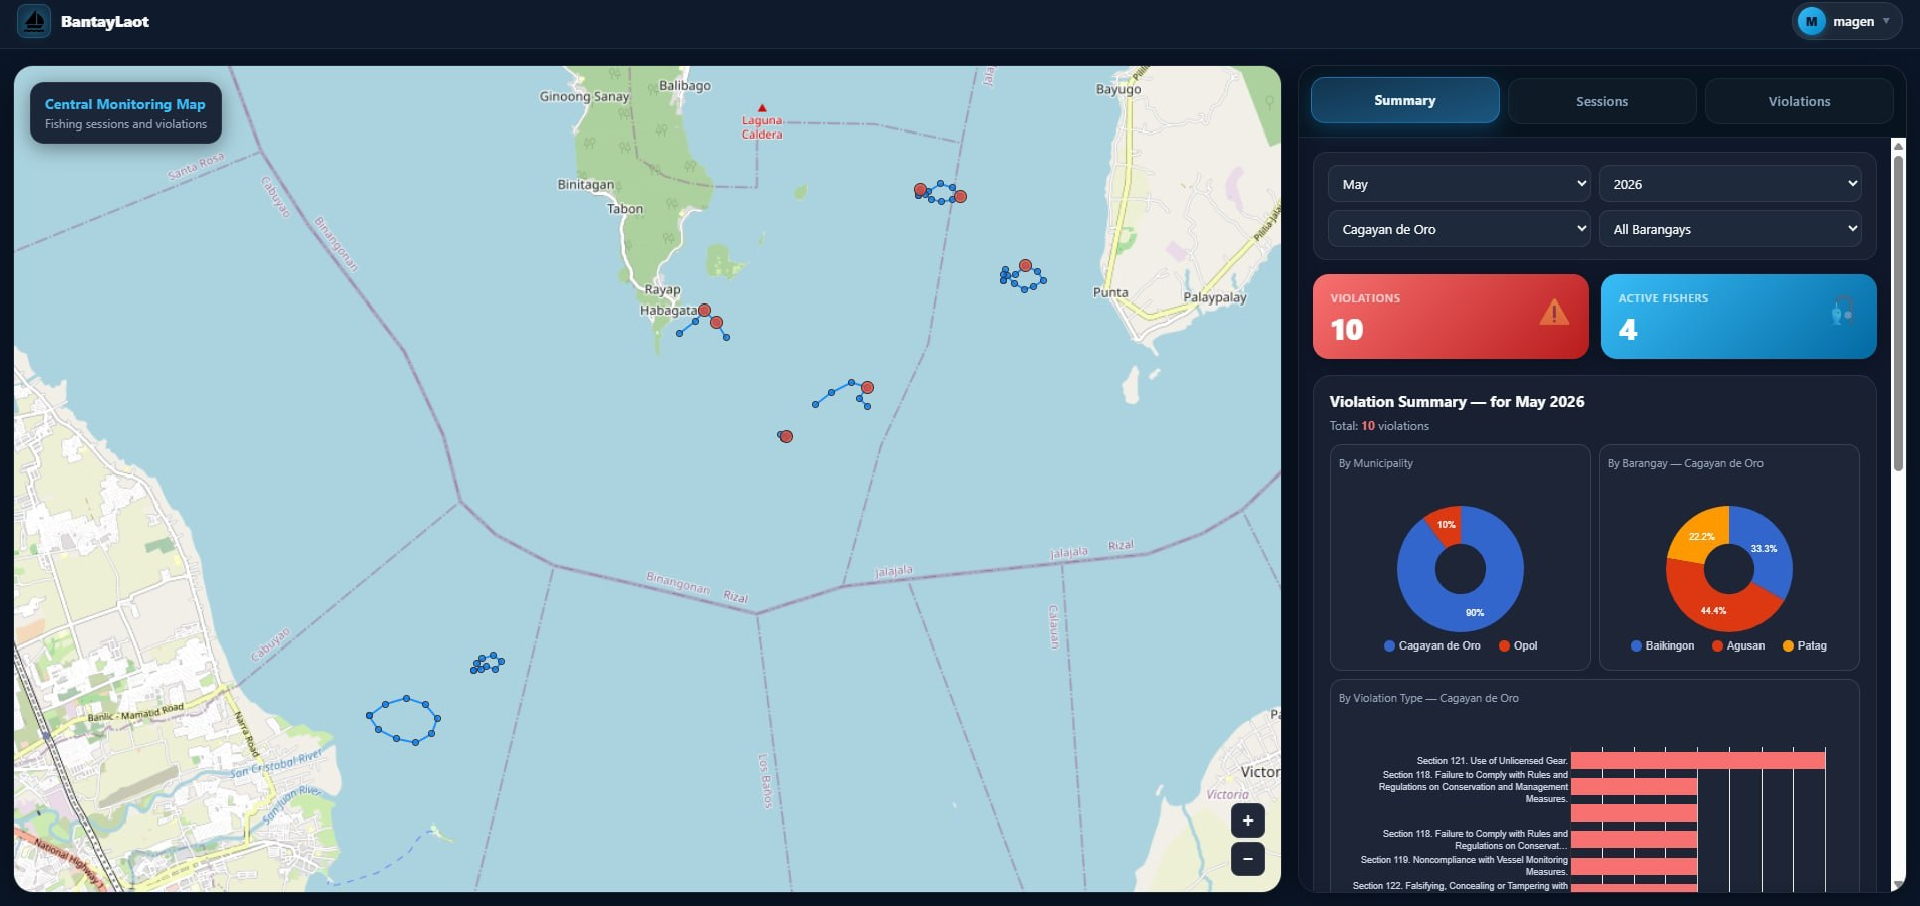
\includegraphics[width=0.45\textwidth]{web_central_overview.jpg}
    \caption{Web Application --- Central Administrator Summary Tab}
    \label{fig:web_central_overview}
\end{figure}

\begin{figure}[h]
    \centering
    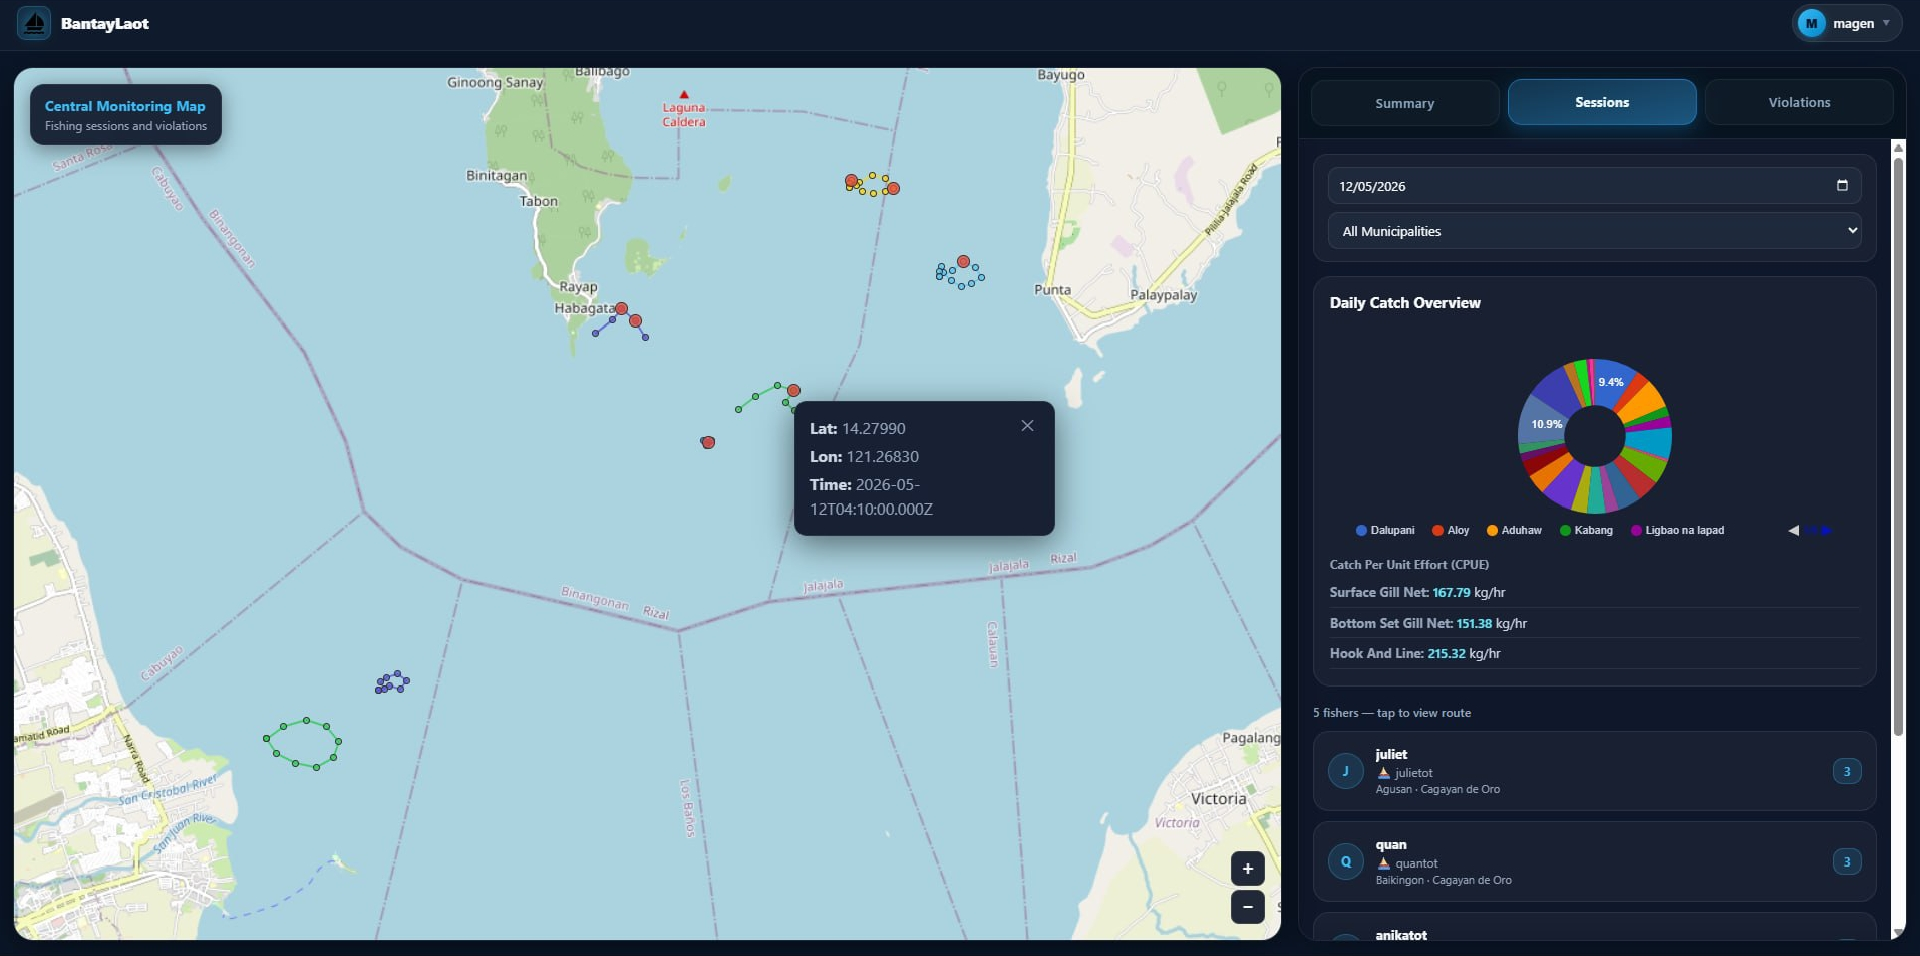
\includegraphics[width=0.45\textwidth]{web_central_cpue.jpg}
    \caption{Web Application --- Sessions Tab with Cross-Municipality Fisher Cards
             (Central View)}
    \label{fig:web_central_cpue}
\end{figure}

The central administrator dashboard, depicted in Fig.~\ref{fig:web_central_overview},
aggregates data from both municipal MongoDB instances via the Railway-hosted central API
and follows the same three-tab layout as the municipal dashboard, extended by a
municipality selector at the filter level. In the Summary Tab, selecting a municipality
causes the violation section to render two side-by-side pie charts---one grouping
violations across all municipalities and one breaking them down by barangay within the
selected municipality---alongside the violation type bar chart. The CPUE card retains
the same species pie chart and expandable fisher breakdown, with each fisher card now
labelled by both barangay and municipality of origin.

The Sessions Tab (Fig.~\ref{fig:web_central_cpue}) presents the same session browsing
experience as the municipal view---date, municipality, and barangay filters; a daily
fish catch overview; fisher cards with session counts; and expandable session detail
with catch analysis and GPS route map---extended to cover all municipalities. The
Violations Tab mirrors this structure, giving central administrators a cross-municipality
view of violation records with the same date, municipality, and barangay filtering and
card expansion available in the municipal dashboard.

Account provisioning is also managed from the Manage Users page, which in the central
administrator context allows creation of researcher accounts and municipal administrator
accounts directly, without requiring self-registration. The user table in this view
spans all municipalities and includes a municipality column, giving central administrators
a complete roster of registered users across the deployment.

\subsubsection{Researcher Dashboard}

\begin{figure}[h]
    \centering
    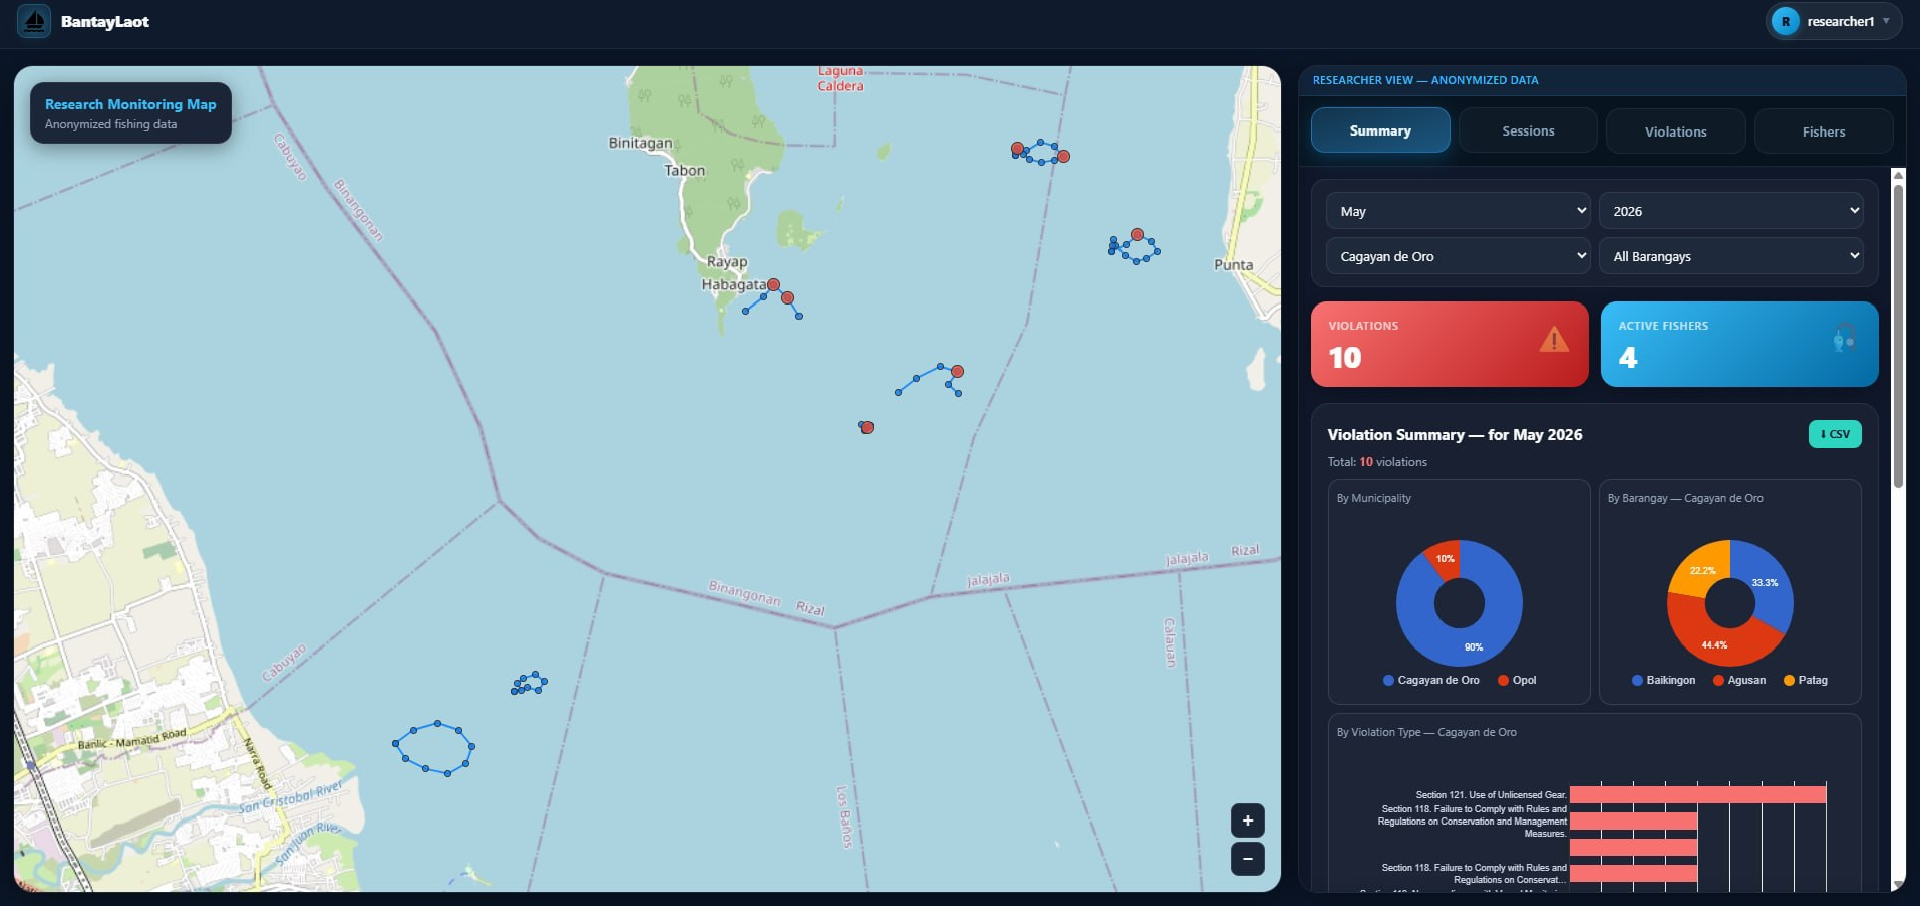
\includegraphics[width=0.45\textwidth]{web_researcher_summary.jpg}
    \caption{Web Application --- Researcher Summary Tab}
    \label{fig:web_researcher_summary}
\end{figure}

\begin{figure}[h]
    \centering
    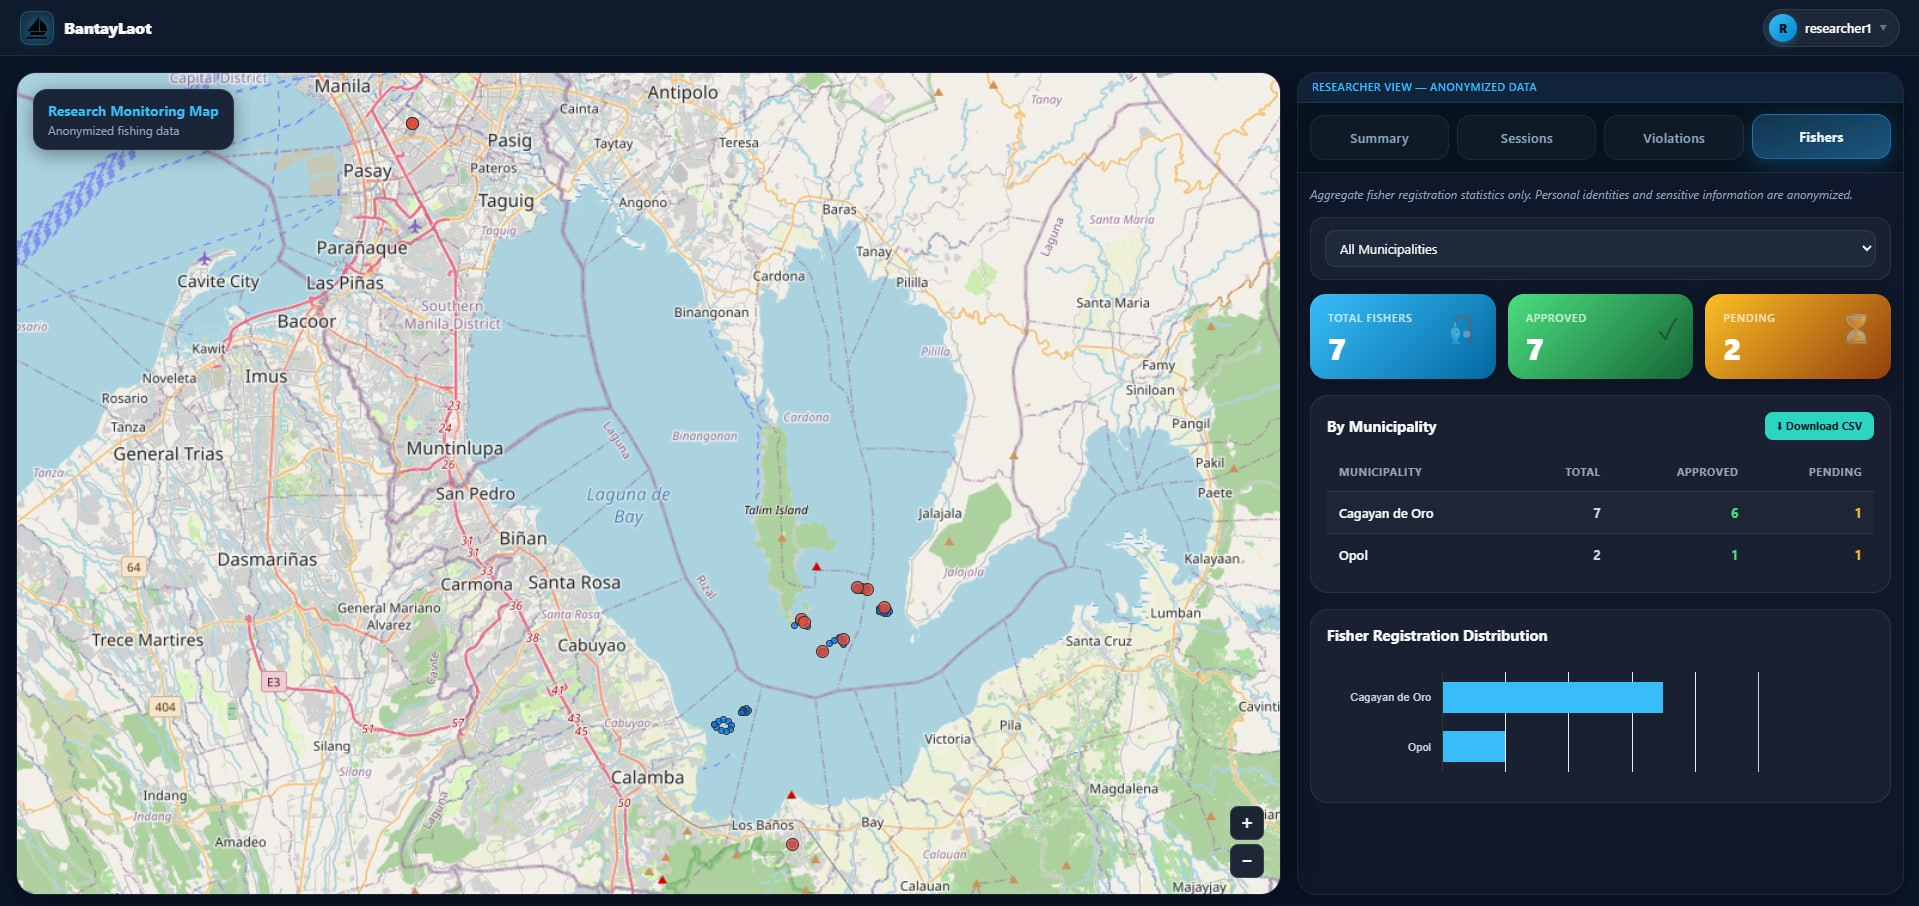
\includegraphics[width=0.45\textwidth]{web_researcher_fishers.jpg}
    \caption{Web Application --- Researcher Fishers Tab}
    \label{fig:web_researcher_fishers}
\end{figure}

The researcher dashboard presents anonymized fisheries data across four tabs: Summary,
Sessions, Violations, and Fishers. As shown in Fig.~\ref{fig:web_researcher_summary},
the Summary Tab replicates the central administrator layout---month, year, municipality,
and barangay filters; violation pie charts; violation type bar chart; species catch pie
chart; and per-gear CPUE row---but adds a Download CSV button to both the Violation
Summary card and the CPUE card, enabling export of the displayed monthly aggregates.
No fisher names or identifying details appear anywhere in the researcher view. The
Sessions and Violations tabs follow the same pattern as the central equivalents, each
with Download CSV and Download Images buttons and individual image download controls
within detail views. Violation records expose gear type, vessel description, origin
area, GPS coordinates, and timestamp, but omit reporter and violator identities.

The Fishers Tab (Fig.~\ref{fig:web_researcher_fishers}), unique to the researcher
role, provides aggregate fisher registration statistics. Three stat cards at the top
display counts of total registered fishers, approved accounts, and pending accounts.
Below, a sortable table groups registrations by municipality; selecting a municipality
from the filter switches the table to a barangay-level breakdown within that
municipality, with Total, Approved, and Pending columns. A Google Charts bar chart
renders the same distribution visually, and a Download CSV button exports the
displayed counts. A note within the tab confirms that personal identities and
sensitive information are excluded from this view.

\subsection{Technical Difficulties}

Development of BantayLaot+ encountered several technical challenges arising from the
system's offline-first requirements, multi-tier data architecture, and cross-origin
deployment configuration. These are documented as they directly informed design decisions
described in the methodology.

\subsubsection{Room Database Schema Design for Sync State Management}

Managing three distinct synchronization states (PENDING, SYNCED, FAILED) across multiple
entity types---sessions, catches, violations, and GPS tracks---required careful schema
iteration. Early designs used a single global sync flag per record, which proved
insufficient for partial-upload scenarios where metadata was successfully transmitted but
the associated image failed due to payload constraints. The schema was revised to track
image URI sync status independently from record metadata, allowing the system to resume
interrupted uploads without retransmitting already-synced fields or duplicating data.

\subsubsection{WorkManager Constraint Configuration}

Configuring WorkManager to queue synchronization reliably while avoiding spurious retries
required careful coordination of constraint and work policies. All sync tasks---sessions,
catches, violations, GPS tracks, and images---use a single \texttt{NetworkType.CONNECTED}
constraint, meaning uploads are queued but held until any network connection is available.
The one-time upload worker triggered by the Upload button uses
\texttt{ExistingWorkPolicy.REPLACE}, ensuring that tapping the button while a sync is
already running restarts the operation with the latest stored credentials. The periodic
background worker uses \texttt{ExistingPeriodicWorkPolicy.KEEP} to prevent duplicate
background tasks from accumulating across app restarts.

\subsubsection{JWT Token Persistence and Offline Session Continuity}

Maintaining authenticated sessions during extended field operations required ensuring that
JWT tokens persisted in SharedPreferences remained available for offline use. Fishing
trips in the target Misamis Oriental municipalities could exceed 12 hours without cellular access. Because
the application reads the stored token from SharedPreferences for every API request and
does not require a live server check to load the home screen, users remain logged in and
can record sessions, catches, violations, and GPS tracks without connectivity. The token
is sent to the server only during the actual upload, at which point a valid network
connection is already required by the WorkManager constraint.

\subsubsection{GPS Data Volume and Battery Optimization}

Recording GPS fixes at 30-second intervals across multi-hour sessions generated
substantial data volumes; a single 10-hour trip produces approximately 1,200 GPS records.
To reduce battery consumption during extended trips, GPS acquisition was implemented as a
foreground service (\texttt{GPSLocationService}) rather than continuous foreground polling,
with the location client receiving updates from the Fused Location Provider at the
configured interval. This approach allows the operating system to manage location hardware
duty cycling while the service remains active, measurably reducing battery consumption
during extended trips.

\subsubsection{Image Compression and Upload Pipeline}

Violation and catch photographs captured at full device resolution produced files ranging
from 3--8~MB per image, making direct upload impractical over intermittent connections.
An image compression pipeline was implemented using Android's Bitmap API within the
SyncWorker to scale captures to a maximum dimension of 1024~px at 70\% JPEG quality
before base64 encoding and transmission. This significantly reduces payload size relative
to raw device captures, enabling reliable transfer under limited bandwidth while
preserving sufficient detail for the evidence photographs visible in
Fig.~\ref{fig:web_munic_violations} and for future AI model training.

\subsubsection{CORS Configuration for Multi-Origin API Communication}

The web application communicates with both the Railway-hosted central API and the
localhost municipal APIs, which present different origins to the browser. CORS policies
on the Express.js servers initially rejected cross-origin requests from the web client's
domain. Each municipal server's CORS configuration was updated to allow all origins,
enabling the cross-origin data access required across all three web dashboard views
(Figs.~\ref{fig:web_munic_overview}, \ref{fig:web_central_overview},
and \ref{fig:web_researcher_summary}). The Railway central API was updated
equivalently.

\subsubsection{MongoDB Deduplication During Sync}

When mobile clients submitted records to the municipal server, duplicate entries could
arise if the upload was retried after a partial success. Each record carries a
\texttt{localId} field assigned at creation time in Room Database. The municipal server
uses MongoDB upsert operations keyed on \texttt{localId}, ensuring that resubmitting an
already-synced record updates the existing document rather than creating a duplicate.
The central aggregation server applies the same upsert strategy when receiving bulk data
from municipal servers, maintaining idempotent ingestion across the full synchronization
pipeline.

\subsubsection{Web Application to Localhost Municipal API Communication}

A significant architectural limitation emerged during deployment: the React web
application cannot directly reach the municipal localhost APIs when accessed from outside
the local network, as localhost resolves to the client browser's own machine rather than
the municipal server. This was addressed by configuring the municipal APIs to bind to the
local area network (LAN) IP address of the on-site machine, making the endpoints
reachable to devices on the same network. This constraint directly affects the municipal
dashboard views shown in
Figs.~\ref{fig:web_munic_overview}--\ref{fig:web_munic_users}, which depend on
the municipal API for jurisdiction-specific data. A reverse proxy configuration was
documented for future implementation. This limitation is acknowledged as a deployment
constraint in the current version and is listed in the recommendations as a candidate for
replacement with cloud-hosted municipal servers.

\subsection{System Usability Evaluation Results}

Usability evaluation was conducted with fifteen respondents drawn from the target user
groups of the two Misamis Oriental municipalities. Five respondents per platform completed
representative task sequences on their assigned system component and rated all ten SUS
items immediately afterward. Results are
presented in Tables~\ref{tab:sus_mobile}, \ref{tab:sus_municipal}, and
\ref{tab:sus_researcher}.

\subsubsection{Mobile Application (n = 5)}

\begin{table}[h]
\centering
\caption{SUS Results --- Mobile Application}
\label{tab:sus_mobile}
\begin{tabular}{@{}cc@{}}
\toprule
\textbf{Respondent} & \textbf{SUS Score} \\
\midrule
Respondent 1 & 100.0 \\
Respondent 2 & 80.0 \\
Respondent 3 & 100.0 \\
Respondent 4 & 97.5 \\
Respondent 5 & 100.0 \\
\midrule
\textbf{Average} & \textbf{95.5} \\
\bottomrule
\end{tabular}
\end{table}

\subsubsection{Municipal Administrator Dashboard (n = 5)}

\begin{table}[h]
\centering
\caption{SUS Results --- Municipal Administrator Dashboard}
\label{tab:sus_municipal}
\begin{tabular}{@{}cc@{}}
\toprule
\textbf{Respondent} & \textbf{SUS Score} \\
\midrule
Respondent 1 & 60.0 \\
Respondent 2 & 90.0 \\
Respondent 3 & 92.5 \\
Respondent 4 & 92.5 \\
Respondent 5 & 100.0 \\
\midrule
\textbf{Average} & \textbf{87.0} \\
\bottomrule
\end{tabular}
\end{table}

\subsubsection{Researcher Dashboard (n = 5)}

\begin{table}[h]
\centering
\caption{SUS Results --- Researcher Dashboard}
\label{tab:sus_researcher}
\begin{tabular}{@{}cc@{}}
\toprule
\textbf{Respondent} & \textbf{SUS Score} \\
\midrule
Respondent 1 & 97.5 \\
Respondent 2 & 90.0 \\
Respondent 3 & 85.0 \\
Respondent 4 & 92.5 \\
Respondent 5 & 92.5 \\
\midrule
\textbf{Average} & \textbf{91.5} \\
\bottomrule
\end{tabular}
\end{table}

\subsection{Discussion}

The successful implementation of BantayLaot+ demonstrates that an offline-first fisheries
monitoring architecture is technically feasible within the hardware and connectivity
constraints of Philippine coastal municipalities. The combination of Room Database and
WorkManager proved effective for local data persistence and deferred synchronization,
directly addressing the primary gap identified in the predecessor system. JWT token
persistence resolved offline authentication continuity, enabling extended field use
without connectivity dependency---a critical requirement given trip durations that
routinely exceed mobile network coverage windows in the target municipalities.

The Cloudinary image pipeline established during development is designed to serve as the
initial training dataset infrastructure for future species identification model
development once field deployment is initiated. The catch documentation workflow---photo
capture followed by manual species and weight entry as shown in
Figs.~\ref{fig:mobile_catch}---maps directly onto the
annotation workflow that supervised learning model training would require, and the
existing data schema was designed to accommodate a future AI classification backend
without structural changes.

The technical difficulties encountered during development---particularly those related to
CORS configuration for multi-origin communication and the LAN-dependency constraint for
municipal API access---highlight architectural limitations that should be resolved before
scaling deployment to additional municipalities. The recommendation to replace on-site
localhost servers with cloud-hosted municipal instances would eliminate both the CORS
origin management burden and the LAN dependency, significantly simplifying the deployment
footprint and enabling full remote administration of the municipality-level dashboards
shown in Figs.~\ref{fig:web_munic_overview}--\ref{fig:web_munic_users}.

SUS evaluation results indicate strong usability across all three platforms. The mobile
application received an average SUS score of 95.5 (n~=~5), rated \textit{Best
Imaginable} on the Bangor et al.\ adjective scale \cite{Bangor2008}, with individual
scores ranging from 80.0 to 100.0. The municipal administrator dashboard achieved an
average of 87.0 (n~=~5), rated \textit{Excellent}, with scores ranging from 60.0 to
100.0; the lower individual score of 60.0 reflects one respondent's unfamiliarity with
the dashboard's scope and layout at first encounter, consistent with their open-ended
comment noting a need for in-app instructions on primary features. The researcher
dashboard received an average of 91.5 (n~=~5), also rated \textit{Best Imaginable},
with individual scores ranging from 85.0 to 97.5. All three averages exceed the 68-point
above-average threshold, and two of three exceed the 80.3-point excellent threshold,
indicating that the session-based mobile workflow, the dropdown-based species selection, the inline upload feedback via the home screen
Upload button, and the role-scoped web views were effective in supporting the target
population's varying digital literacy levels.

Integration testing confirmed that the multi-tiered architecture---mobile client,
localhost municipal server, and cloud central server---is operationally viable at the
intended scale of two municipalities. End-to-end tests verified that catch logs,
violation reports, and GPS tracks are correctly transmitted from the mobile client to the
municipal server and aggregated by the central Railway database, and that the researcher
dashboard (Fig.~\ref{fig:web_researcher_summary}) correctly renders anonymized data
drawn from multiple municipal sources. These outcomes substantiate the architecture's
readiness to support the study's stated objectives of improved offline operation,
structured multi-role data management, and scalable evidence collection for fisheries
enforcement and research upon field deployment.

%% ============================================================
%% SECTION V — CONCLUSION AND RECOMMENDATIONS
%% ============================================================

\section{Conclusion and Recommendations}

BantayLaot+ successfully addresses the operational gaps identified in the predecessor
system, delivering a functional, multi-component fisheries monitoring platform intended
for deployment across two municipalities in Misamis Oriental. The system introduces
JWT-based authentication with offline session continuity, a structured WorkManager
synchronization pipeline with per-record state tracking across sessions, catches,
violations, and GPS tracks, and a multi-tiered server architecture separating
per-municipality and central data stores. Three role-differentiated web dashboards
provide jurisdiction-appropriate analytics for municipal administrators, central
administrators, and researchers, with the researcher dashboard uniquely supporting
anonymized data access and CSV export. A structured Cloudinary image pipeline completes the data collection framework,
establishing the infrastructure for future AI-assisted species identification without
requiring schema changes.

The deployment architecture also demonstrates practical feasibility in terms of
operational cost. The centralized cloud server hosted on Railway is estimated to cost
approximately USD 5--20 per month depending on database usage, storage, and server
uptime requirements, while Cloudinary usage for image storage and delivery may remain
within the free-tier allocation during early deployment stages, with estimated scaling
costs beginning at approximately USD 25 per month for larger image datasets and higher
API usage. These costs suggest that the system remains financially viable for local
government deployment and future scaling.

SUS evaluation with fifteen respondents across three user groups returned average scores
of 95.5 (mobile application, \textit{Best Imaginable}), 87.0 (municipal administrator
dashboard, \textit{Excellent}), and 91.5 (researcher dashboard, \textit{Best
Imaginable}), all exceeding the above-average usability threshold of 68 \cite{Bangor2008}.
These results indicate that the interface design is appropriate for the target
population's varying digital literacy levels. Integration testing confirmed end-to-end
data flow from the mobile client through the municipal server to the central Railway
database, substantiating the multi-tiered architecture's readiness to support the study's
stated objectives upon field deployment.

Recommended directions for future work include:
\begin{itemize}
    \item Implementing the AI-assisted fish species identification and weight estimation
    module using the image dataset collected through deployment.
    \item Expanding deployment to additional municipalities and evaluating scalability of
    the localhost-to-Railway synchronization architecture under higher data volumes.
    \item Replacing localhost municipal servers with cloud-hosted instances to eliminate
    dependency on on-site hardware and improve availability.
\end{itemize}

%% ============================================================
%% BIBLIOGRAPHY
%% ============================================================

\begin{thebibliography}{99}

\bibitem{Bangor2008}
A. Bangor, P. T. Kortum, and J. T. Miller, ``An empirical evaluation of the System
Usability Scale,'' \textit{International Journal of Human-Computer Interaction},
vol. 24, no. 6, pp. 574--594, 2008.

\bibitem{Alzubaidi2020}
L. Alzubaidi, ``Designing REST APIs for scalable distributed systems,'' ResearchGate,
2020.

\bibitem{Chodorow2013}
K. Chodorow, \textit{MongoDB: The Definitive Guide}. Sebastopol, CA: O'Reilly Media,
2013.

\bibitem{Dahiru2021}
A. Dahiru and M. Ibrahim, ``Offline authentication approaches for secure mobile
systems,'' \textit{International Journal of Computer Applications}, vol. 183, no. 24,
2021.

\bibitem{FAO2023}
Food and Agriculture Organization, \textit{The State of World Fisheries and Aquaculture}.
Rome: FAO Publishing, 2023.

\bibitem{Gallero2025}
J. Gallero, ``BantayLaot: A mobile-based fisheries monitoring system for municipal
waters,'' \textit{Philippine Journal of ICT for Development}, vol. 9, no. 1,
pp. 22--38, 2025.

\bibitem{Goncalves2020}
J. Goncalves, D. Ferreira, and V. Kostakos, ``Mobile crowdsensing and data
synchronization challenges in developing regions,'' \textit{IEEE Pervasive Computing},
vol. 19, no. 3, 2020.

\bibitem{Google2022}
Google Developers, ``Why Kotlin is the preferred language for Android,'' 2022.
[Online]. Available: https://developer.android.com/kotlin

\bibitem{Haklay2008}
M. Haklay and P. Weber, ``OpenStreetMap: User-generated street maps,''
\textit{IEEE Pervasive Computing}, vol. 7, no. 4, 2008.

\bibitem{Kumar2020}
R. Kumar and M. Singh, ``Synchronization strategies in distributed mobile systems,''
\textit{Journal of Systems Architecture}, vol. 104, 2020.

\bibitem{Norouzzadeh2018}
M. S. Norouzzadeh \textit{et al.}, ``Automatically identifying animal species in camera
trap images,'' \textit{Proceedings of the National Academy of Sciences}, vol. 115,
no. 25, 2018.

\bibitem{Serrano2020}
M. Serrano \textit{et al.}, ``Offline-first approaches for resilient mobile
applications,'' \textit{ACM Computing Surveys}, vol. 53, no. 6, 2020.

\bibitem{WWF2022}
World Wildlife Fund, \textit{IUU Fishing Facts and Impacts on Global Fisheries}.
WWF Oceans Report, 2022.

\end{thebibliography}

\end{document}
